% Options for packages loaded elsewhere
\PassOptionsToPackage{unicode}{hyperref}
\PassOptionsToPackage{hyphens}{url}
\PassOptionsToPackage{dvipsnames,svgnames,x11names}{xcolor}
%
\documentclass[
  letterpaper,
  DIV=11,
  numbers=noendperiod]{scrartcl}

\usepackage{amsmath,amssymb}
\usepackage{setspace}
\usepackage{iftex}
\ifPDFTeX
  \usepackage[T1]{fontenc}
  \usepackage[utf8]{inputenc}
  \usepackage{textcomp} % provide euro and other symbols
\else % if luatex or xetex
  \usepackage{unicode-math}
  \defaultfontfeatures{Scale=MatchLowercase}
  \defaultfontfeatures[\rmfamily]{Ligatures=TeX,Scale=1}
\fi
\usepackage{lmodern}
\ifPDFTeX\else  
    % xetex/luatex font selection
\fi
% Use upquote if available, for straight quotes in verbatim environments
\IfFileExists{upquote.sty}{\usepackage{upquote}}{}
\IfFileExists{microtype.sty}{% use microtype if available
  \usepackage[]{microtype}
  \UseMicrotypeSet[protrusion]{basicmath} % disable protrusion for tt fonts
}{}
\usepackage{xcolor}
\setlength{\emergencystretch}{3em} % prevent overfull lines
\setcounter{secnumdepth}{5}
% Make \paragraph and \subparagraph free-standing
\ifx\paragraph\undefined\else
  \let\oldparagraph\paragraph
  \renewcommand{\paragraph}[1]{\oldparagraph{#1}\mbox{}}
\fi
\ifx\subparagraph\undefined\else
  \let\oldsubparagraph\subparagraph
  \renewcommand{\subparagraph}[1]{\oldsubparagraph{#1}\mbox{}}
\fi


\providecommand{\tightlist}{%
  \setlength{\itemsep}{0pt}\setlength{\parskip}{0pt}}\usepackage{longtable,booktabs,array}
\usepackage{calc} % for calculating minipage widths
% Correct order of tables after \paragraph or \subparagraph
\usepackage{etoolbox}
\makeatletter
\patchcmd\longtable{\par}{\if@noskipsec\mbox{}\fi\par}{}{}
\makeatother
% Allow footnotes in longtable head/foot
\IfFileExists{footnotehyper.sty}{\usepackage{footnotehyper}}{\usepackage{footnote}}
\makesavenoteenv{longtable}
\usepackage{graphicx}
\makeatletter
\def\maxwidth{\ifdim\Gin@nat@width>\linewidth\linewidth\else\Gin@nat@width\fi}
\def\maxheight{\ifdim\Gin@nat@height>\textheight\textheight\else\Gin@nat@height\fi}
\makeatother
% Scale images if necessary, so that they will not overflow the page
% margins by default, and it is still possible to overwrite the defaults
% using explicit options in \includegraphics[width, height, ...]{}
\setkeys{Gin}{width=\maxwidth,height=\maxheight,keepaspectratio}
% Set default figure placement to htbp
\makeatletter
\def\fps@figure{htbp}
\makeatother

\usepackage{fontspec}
\usepackage{multirow}
\usepackage{multicol}
\usepackage{colortbl}
\usepackage[normalem]{ulem}
\usepackage{hhline}
\newlength\Oldarrayrulewidth
\newlength\Oldtabcolsep
\usepackage{longtable}
\usepackage{array}
\usepackage{hyperref}
\usepackage{float}
\usepackage{wrapfig}
% \usepackage{hyperref}
% \hypersetup{
%     colorlinks,
%     linkcolor={blue!100!black},
%     citecolor={blue!100!black},
%     urlcolor={blue!100!black}
% }
% \usepackage{apacite}
% \usepackage[round]{natbib} 
% \usepackage{graphicx}
% \usepackage{float}
% \usepackage{caption}
% \usepackage[toc,page]{appendix}
% \usepackage{booktabs,caption}
% \usepackage[flushleft]{threeparttable}
% \usepackage{tabularx}
% Figure note command: compact font + tighter leading, prefixes "Note:"
\newcommand{\fignote}[1]{%
  \vspace{-0.5em}%
  {\scriptsize\linespread{1.1}\selectfont\noindent\textit{Note:}~#1\par}%
}
\usepackage{sfmath}
\usepackage{fontspec}
\usepackage[utf8]{inputenc}
\usepackage{siunitx}
\usepackage{amsfonts}
\usepackage{amsmath}
% \usepackage{xcolor}
% \usepackage{scrextend}
% \deffootnote[2em]{2em}{1em}{\textsuperscript{\thefootnotemark}\,}
% \newcolumntype{Y}{>{\centering\arraybackslash}X}
% \usepackage[a4paper]{geometry}
% \usepackage{caption}
% \usepackage[bottom,flushmargin,hang,multiple]{footmisc}
% \usepackage{pdflscape}
% \usepackage[paper=portrait,pagesize]{typearea}
% \usepackage{rotating}
% \usepackage{fullpage}
% \usepackage{tabu}
\usepackage{lscape}
\newcommand{\blandscape}{\begin{landscape}}
\newcommand{\elandscape}{\end{landscape}}
\usepackage{rotating}
\newcommand{\bsideways}{\begin{sidewaystable}[htbp]}
\newcommand{\esideways}{\end{sidewaystable}}
\let\oldsection\section
\renewcommand\section{\oldsection}
\KOMAoption{captions}{tableheading}
\makeatletter
\@ifpackageloaded{caption}{}{\usepackage{caption}}
\AtBeginDocument{%
\ifdefined\contentsname
  \renewcommand*\contentsname{Table of contents}
\else
  \newcommand\contentsname{Table of contents}
\fi
\ifdefined\listfigurename
  \renewcommand*\listfigurename{List of Figures}
\else
  \newcommand\listfigurename{List of Figures}
\fi
\ifdefined\listtablename
  \renewcommand*\listtablename{List of Tables}
\else
  \newcommand\listtablename{List of Tables}
\fi
\ifdefined\figurename
  \renewcommand*\figurename{Figure}
\else
  \newcommand\figurename{Figure}
\fi
\ifdefined\tablename
  \renewcommand*\tablename{Table}
\else
  \newcommand\tablename{Table}
\fi
}
\@ifpackageloaded{float}{}{\usepackage{float}}
\floatstyle{ruled}
\@ifundefined{c@chapter}{\newfloat{codelisting}{h}{lop}}{\newfloat{codelisting}{h}{lop}[chapter]}
\floatname{codelisting}{Listing}
\newcommand*\listoflistings{\listof{codelisting}{List of Listings}}
\makeatother
\makeatletter
\makeatother
\makeatletter
\@ifpackageloaded{caption}{}{\usepackage{caption}}
\@ifpackageloaded{subcaption}{}{\usepackage{subcaption}}
\makeatother
\ifLuaTeX
  \usepackage{selnolig}  % disable illegal ligatures
\fi
\usepackage[round]{natbib}
\bibliographystyle{apalike}
\usepackage{bookmark}

\IfFileExists{xurl.sty}{\usepackage{xurl}}{} % add URL line breaks if available
\urlstyle{same} % disable monospaced font for URLs
\hypersetup{
  colorlinks=true,
  linkcolor={blue!000!black},
  filecolor={Maroon},
  citecolor={blue!000!black},
  urlcolor={blue!000!black},
  pdfcreator={LaTeX via pandoc}}

\author{}
\date{}

\begin{document}

\title{The Climate Credit Channel: Physical Shocks and Monetary Policy Transmission in South Africa}





\author { Tichinashe Mabugu\footnote{Corresponding Author. Economic Research Department, South African Reserve Bank; Email: xolani.sibande@resbank.co.za} \and Xolani Sibande\footnote{Economic Research Department, South African Reserve Bank; Email: tichinashe.mabugu@resbank.co.za.}} 


\date{\today}
\maketitle

\begin{abstract}
AAAAAA

\end{abstract}

\noindent\textbf{Keywords}: \\
\textbf{JEL Codes}: 
\newpage

\setstretch{1.5}
\section{Introduction}\label{introduction}

The credit channel is a central mechanism through which monetary policy
reaches the real economy. By altering the external finance premium ---
the wedge between the cost of internal and external funds generated by
credit-market frictions --- monetary policy shifts the borrowing costs
and balance sheet positions of both firms and households, with
downstream effects on investment, consumption, and ultimately output and
prices \citep{bernanke1995}. Two linkages underpin this transmission:
the balance sheet channel, which operates through changes in borrower
net worth and collateral values, and the bank lending channel, which
operates through the supply of loanable funds \citep{hall2001}.
Considerable empirical evidence has established the balance sheet
channel as quantitatively important in advanced economies
\citep{aysun2013, altavilla2024, ashcraft2007}, yet a full accounting of
its strength remains elusive, particularly in emerging markets where the
institutional context differs markedly from the settings in which most
of this evidence was gathered \citep{pirozhkova2025}.

A related challenge is that observed credit responses to monetary policy
do not always conform to the predictions of standard transmission
models. Information effects, heterogeneous bank balance sheets, and the
distinction between anticipated and unanticipated rate changes all
generate dispersion in the pass-through of policy to credit conditions
\citep{ALTAVILLA202081, KLEIMEIER20061839}. This motivated the
development of structural monetary policy surprise measures ---
residuals purged of the component of rate changes that can be predicted
from the central bank's own information set, or from financial market
expectations --- which isolate the genuinely unexpected component of
policy \citep{romer2004, miyajima2024}. It is precisely this unexpected
component, by definition unconfounded by the macroeconomic conditions
that prompted the rate decision, that permits causal inference about the
credit channel. Yet even with carefully identified surprise measures,
the literature documents atypical and heterogeneous responses that
standard models struggle to rationalise, suggesting that the full set of
factors shaping credit channel strength is not yet well understood.

This paper proposes that physical climate shocks constitute one such
factor. Climate shocks --- deviations of temperature and precipitation
from their long-run seasonal norms --- affect firms and households
through channels that closely mirror the determinants of the external
finance premium: they disrupt production, damage capital and collateral,
compress profitability, and erode net worth
\citep{dafermos2018, aglietta2016}. If such damage coincides with a
monetary policy tightening, the deterioration in borrower balance sheets
may amplify the credit response --- lending rates rising further or
credit volumes contracting more sharply than the policy shock alone
would produce. Alternatively, if a benign climate shock supports
economic activity at the same moment that policy tightens, it may
cushion the credit response and dampen the effectiveness of monetary
policy. The direction and magnitude of this interaction is an empirical
question, and one that has received limited attention despite its clear
implications for how central banks should interpret the transmission of
their decisions.

The specific question this paper investigates is: does the coincidence
of physical climate shocks with monetary policy surprises alter the
strength and direction of credit channel transmission in South Africa?
Concretely, when a temperature or precipitation shock accompanies an
unexpected tightening, are lending rates kept higher for longer, or is
the rate response muted? Do credit volumes contract more sharply, or
does climate-driven demand for borrowing offset the policy impulse? We
examine both amplification --- in which climate shocks strengthen the
credit response to monetary policy --- and dampening --- in which they
weaken it --- across six monetary policy surprise measures, two climate
shock variables, and twelve disaggregated credit series covering
corporate and household borrowers at the bank level. South Africa
provides a particularly informative setting: it is a climate-vulnerable
emerging economy with well-developed financial markets, a credible
independent central bank, and granular bank-level credit data
disaggregated by borrower type and product that is rarely available in
comparable economies.

Using bank-level panel data over 2011--2025 and a combination of panel
fixed effects regressions and panel local projections, we find that the
interaction between climate and monetary policy shocks operates
primarily through the price of credit --- lending rates --- rather than
its quantity, consistent with a risk-repricing mechanism. The effects
are heterogeneous across shock types and credit products, with
amplification and dampening both present depending on the specific
climate and monetary policy pairing. They are also persistent, with the
interaction peaking at 8--10 quarters after the shock and most
pronounced under extreme climate conditions at the tails of the
distribution. These findings point to physical climate risk as a
systematic but previously underappreciated source of variation in the
strength of the credit channel, with implications for how
climate-vulnerable central banks model and communicate monetary policy
transmission.

The remainder of the paper is organised as follows. Section 2 develops
the conceptual framework linking climate shocks to the external finance
premium. Section 3 describes the data and methodology, including the
construction of the monetary policy surprise and climate shock series.
Section 4 presents the main fixed effects and local projection results.
Section 5 examines heterogeneity across shock types, credit products,
and climate intensity. Section 6 concludes.

\section{Conceptual Framework}\label{conceptual-framework}

We argue that climate shocks may alter the strength of the credit
channel by affecting the financial position of corporates, households
and banks. For simplicity, we illustrate the transmission of a
contractionary monetary policy shock through the credit channel
throughout this section. We distinguish between two possible effects
that can ensue when a monetary policy shock coincides with a climate
shock: amplification and dampening. We define amplification as a
strengthening of the response of corporates or households to a monetary
policy shock, such that the response of credit rates or volumes moves in
the same direction as the response to the monetary policy shock alone,
but with a larger absolute magnitude when the climate shock is present.
A dampening effect, in contrast, occurs when the response continues to
move in the same direction as the response to the monetary policy shock
alone, but with a smaller absolute magnitude when the climate shock is
present.

\subsection{Corporates}\label{corporates}

From the perspective of corporates, we draw from a framework put forward
by \citet{Bean2002Financial} as follows:
\begin{equation}\phantomsection\label{eq-corporate_interest_rate}{
R_{it}^{c} = R_t + f(D_t/E_t), \qquad f' > 0
}\end{equation}

where \(R_{it}^{c}\) is the interest rate faced by corporates which is
dependent on \(R_t\), the risk-free interest rate and a function of the
corporate's financial position, in this case represented by its Debt
(\(D_t\)) to Equity (\(E_t\)) ratio. This function, \(f\) therefore
represents the external finance premium. Insofar as there are
information asymmetries or financial frictions,
Equation~\ref{eq-corporate_interest_rate} holds.

We posit that climate shocks alter the interest rate faced by corporates
through changes in their financial position, which affect the external
finance premium and, consequently, the cost of borrowing
\citep{LAUMER2025104949}. In particular, a climate shock can yield
supply chain disruptions, damage of capital and production losses. These
effects may reduce revenue and profits. Simultaneously, climate
shock-related damage may reduce the value of collateral against which
corporates borrow. These effects can increase corporate debt, \(D_t\),
while the associated decline in profitability, asset values and net
worth can reduce equity, \(E_t\). Consequently, a climate shock may
increase a corporate's finance premium and in turn, raise the cost of
external finance faced by the corporate. In this way, an adverse climate
shock amplifies a contractionary monetary policy shock.

The same framework allows for a dampening effect of contractionary
monetary policy. That is, firms with large cash buffers, liquid assets
or adequate insurance coverage may experience little or no deterioration
in their balance sheets, resulting in little or no change in \(D_t/E_t\)
and consequently in the external finance premium, \(f(D_t/E_t)\),
following a climate shock. This resilience can also render corporates
less responsive to the higher borrowing costs. Thus, climate shocks need
not strengthen the transmission of monetary policy and may instead leave
it unchanged or weaken it. Evidence that cash holdings can mitigate the
effect of monetary tightening on corporate investment supports this
mechanism \citep{SharpeSuarez2020}.

A final, related potential propagation mechanism for corporates arises
from the possibility that corporate borrowing and investment decisions
may be relatively less responsive to changes in borrowing costs. If
climate shocks demand a need for adaptation, replacement of capital or
reconstruction, corporates may have a strong incentive to undertake this
investment even when \(R_t\) rises. In this case, corporates may become
less sensitive to the cost of external finance. This does not
necessarily mean that \(R_{it}^{c}\) itself falls; rather, the higher
financing cost has a smaller effect on corporates' borrowing decisions.
This effect would be most evident when higher interest rates coincide
with an increase in credit volumes. Consistent with this possibility,
\citet{XU2025108087} demonstrate that adaptation policy increases firm
investment even in the absence of an easing of financial constraints
faced by firms.

\subsection{Households}\label{households}

Analogous to Equation~\ref{eq-corporate_interest_rate}, we this of
households facing an interest rate according to the following Equation:
\begin{equation}\phantomsection\label{eq-household_interest_rate}{
R_{it}^{h} = R_t + \phi_{t}, \qquad \phi_{t} > 0
}\end{equation} where \(R_{it}^{h}\) is the interest rate faced by
households as a result of the policy rate \(R_t\) and the
household-specific spread between the policy rate and the cost of
borrowing \(\phi_{t}\). The spread can be viewed as reflecting household
creditworthiness, indebtedness, income and collateral and other
characteristics that affect lenders' assessment of credit risk and the
terms at which credit is supplied. Thus, \(\phi_{t}\) allows households
facing the same monetary policy rate to nevertheless face different
borrowing costs. This allowance for differentiated credit market
outcomes faced by households is driven by evidence suggesting that
transmission of monetary policy varies across households according to a
range of factors including their exposure to income fluctuations
\citep{SLACALEK2020103879}.

The household mechanism ensues similarly to the case of firms. On the
one hand, climate shocks may amplify the credit channel's response to
monetary policy shocks. It follows that a climate shock may reduce
household income, wealth or damage collateral. This deterioration in the
balance sheet of households increases the household-specific spread,
\(\phi_{t}\), causing affected households to face higher borrowing costs
for a given monetary policy rate. On the other hand, climate shocks may
dampen this impact in a similar way to the case of corporates. That is
households with liquid assets, insurance coverage or other financial
buffers may be able to absorb climate-related losses without a
deterioration in their financial position or increased reliance on
external finance. In such cases, the climate shock may generate little
change in \(\phi_{t}\) and therefore need not amplify the response of
household borrowing costs to monetary policy.Empirical evidence suggests
that insurance may lower debt levels in the face of disasters as
households use insurance payouts to pay off mortgages rather than to
reconstruct \citep{Household2017}.

\subsection{Banks}\label{banks}

The household and firm mechanisms are connected through the financial
sector. Climate shocks can affect not only borrowers' demand for credit
but also banks' willingness to supply it. There is a possibility that
during climate shock episodes, creditors heighten the importance they
attach to corporates' and households' balance sheet strength. Indeed,
there is evidence that mortgage arreas is higher in regions that have
faced more damage from climate shocks relative to less damaged regions
\citep{HO2023102790} Recent evidence suggests that in response, banks
pose stricter lending conditions to borowers in disaster-prone regions
\citep{Duanmu02012022}.

On the other hand, a climate shock may dampen the transmission of
monetary policy if it reduces the demand for credit. A deterioration in
economic activity following a climate shock or adequate buffers to
climate shocks may weaken corporates' and households' demand for new
borrowing, reducing banks' loan demand and limiting the extent to which
the shock translates into tighter credit conditions. When loan demand is
weaker, banks may have less scope or incentive to adjust lending rates
in response to changes in the riskiness of their borrowers. In this
case, the climate shock may generate little additional increase in the
spread between lending rates and the policy rate, thereby limiting its
potential to amplify the increase in borrowing costs associated with a
monetary policy tightening.

\subsection{Policy}\label{policy}

We must also consider the role that the policy rate, itself, plays in
the determination of credit rates and, by extension, volumes. Two
related concepts influence our framework. The first is around the
mechanics of monetary policy transmission. Monetary policy transmission
to lending rates is notoriously heterogeneous across banks and dependent
on several factors such as bank balance sheet characteristics
\citep{ALTAVILLA202081}.

The second concept relates to the distinction between an anticipated
interest rate change and an unanticipated rate change. Monetary policy
passthrough in the credit market is faster when the policy rate is
correctly anticipated \citep{KLEIMEIER20061839}. We study monetary
policy surprises which, by design, are unanticipated.

This has non-negligible implications for credit condition outcomes. In
particular,\ldots{}

\subsection{Climate Shock
Non-Linearity}\label{climate-shock-non-linearity}

Until now we have assumed that climate shocks yield adverse effects on
corporates, households and banks. This is not necessarily always the
case. Consider the case of precipitation shocks. One of the main ways
that climate shocks impact macroeconomic outcomes is through the
agricultural sector. Agricultural production is reliant on rainfall in
the South African context where the majority of crops are rainfed
\citep{Hartley2021ClimateUncertainty} . This dependence is further
heightened by the country's relatively limited water resources
\citep{GovernmentSouthAfrica2024WaterSanitation}. Hence, non-extreme
positive precipitation shocks may aid agricultural production. This may,
in turn, yield favourable outcomes in the agricultural sector as well as
upstream and downstream sectors and ultimately allow for a reduction in
\(f(D_t/E_t)\) and \(\phi_{t}\).

While we present an array of explanations for how climate shocks
interact with monetary policy transmission, we ultimately focus on
whether the overall responsiveness of credit conditions to monetary
policy shocks changes in the presence of climate shocks, without
attributing this change to a specific household, corporate or
banking-sector mechanism.

\section{Data and methodology}\label{data-and-methodology}

\subsection{Data}\label{data}

The analysis draws on three main data sources: climate shocks, monetary
policy shocks, and credit extension data. The sample covers South Africa
over the period 2011--2025. All series are observed at a quarterly
frequency, determined by the availability of the monetary policy shock
data; higher-frequency series are aggregated to quarterly values by
taking averages or sums where appropriate.

\textbf{Climate data:} Temperature and precipitation data are sourced
from the ERA5 reanalysis dataset produced by the European Centre for
Medium-Range Weather Forecasts\footnote{see
  \url{https://cds.climate.copernicus.eu/datasets/reanalysis-era5-single-levels?tab=overview}}.
ERA5 provides globally gridded, hourly atmospheric estimates at a 31 km
horizontal resolution. Grid-level values are weighted by population and
aggregated to monthly averages over South Africa's land area, from which
we construct climate shock variables that capture deviations from
long-run historical norms in temperature and precipitation.

The climate shocks are calculated as follows:

\begin{equation}\phantomsection\label{eq-weather_shock}{ ClimateShock_{t} =  \dfrac{T_{t} -\overline{T}_{t} }{\sigma(T_{t})}, }\end{equation}

where \(ClimateShock_{t}\) is the temperature or precipitation shock at
time \(t\) and \(T_{t}\) is the observed population-weighted climate
variable. For both temperature and precipitation, \(\overline{T}_{t}\)
is the calendar-month mean computed over the full sample period (e.g.,
the mean of all January values from 2011 to 2025), and \(\sigma(T_{t})\)
is the corresponding within-month standard deviation. The resulting
shock series are shown in Figure~\ref{fig-climate_shocks_data} in the
Appendix.

\textbf{Monetary policy data:} The monetary policy shock series is
constructed using high-frequency policy surprises for South Africa from
\citet{pirozhkova2025}, alongside the repurchase (repo) rate from the
South African Reserve Bank (SARB). The high-frequency surprises serve as
an instrument to purge the endogenous component of policy rate changes,
yielding a shock series that satisfies the exogeneity requirement of the
regression framework described in Section~\ref{sec-methodology}. For
robustness, we consider both market-based shocks from
\citet{pirozhkova2025} (see
Figure~\ref{fig-market_based_surprises_data}) and a theory-based shock
derived from the policy rate, as described in
Section~\ref{sec-methodology} below (see
Figure~\ref{fig-theory_based_surprises_data}). Surprises are timed to
coincide with policy rate announcement dates and aggregated to a
quarterly frequency. Underlying the calculation of the are the forecasts
of the real GDP growth, the policy rate (repo-rate), and the inflation
rate from Bloomberg Consensus.

\textbf{Credit extension data:} Private sector credit extension data ---
disaggregated by borrower type (households and corporates) at the bank
level --- are obtained from the SARB's BA900 and BA930 bank compliance
reports.\footnote{BA930 data at the bank level are not publicly
  available.} These series include both credit volumes and lending
rates, and are constructed following \citet{sibande2025} and
\citet{sibande2025a} by sorting and aggregating individual bank records
into the broad credit categories used in the study: unsecured, secured,
and mortgage credit. We use the log of credit volumes and make no other
transformations to the other credit data. Summary charts are provided in
Figure~\ref{fig-lending_volume_growth_data} and
Figure~\ref{fig-lending_rates}.

\subsection{Methodology}\label{sec-methodology}

\subsubsection{Shock identification}\label{shock-identification}

Rather than using the policy interest rate directly --- which responds
to prevailing economic conditions and is therefore endogenous --- we use
an unexpected change in monetary policy, commonly called a monetary
policy shock, to isolate the causal effect of policy on credit markets
\citep{miyajima2024}. We construct this shock following
\citet{merrino2022}, who adapts the approach of \citet{romer2004} to the
South African context. The idea is to regress the change in the repo
rate forecast on variables that policymakers were already tracking, and
treat whatever is left over --- the part of the rate change that cannot
be explained by those forecasts --- as the true policy surprise.
Formally:

\begin{equation}\phantomsection\label{eq-mp-shock}{
\Delta r_t = \alpha + \tilde{r_t} + \sum_{t=0}^{2} \beta_t \Delta \tilde{y_t} + \sum_{t=0}^{2} \delta_t \tilde{\pi_t} + \varepsilon_t,
}\end{equation}

where \(\Delta r_t\) is the change in the repo rate forecast,
\(\tilde{r_t}\) is the forecasted repo rate, \(\tilde{y_t}\) is the
forecasted real GDP growth rate, and \(\tilde{\pi_t}\) is the forecasted
inflation rate. The residual \(\varepsilon_t\) --- the unexplained part
of the forecast revision --- is our monetary policy shock,
\(\text{MPShock}_{t}\).\footnote{We include forecasts up to two quarters
  ahead to account for the common assumption among forecasters that
  policy is unchanged in the very near term. See \citet{romer2004} for
  details.}

As an alternative, we construct a second measure of the monetary policy
surprise following \citet{miyajima2024}. This approach uses forecast
errors --- the gap between what forecasters expected and what actually
occurred --- rather than SARB forecasts. The construction proceeds in
two steps. First, for each variable \(i\), the forecast error is:

\begin{equation}\phantomsection\label{eq-forecast_error}{
FE^i_{t} =  EXP^i_{t} - ACT^i_{t},
}\end{equation}

where
\(i \in \{\text{policy rate}, \text{inflation}, \text{GDP growth}\}\),
\(ACT^i_{t}\) is what was actually observed, and \(EXP^i_{t}\) is the
Bloomberg consensus forecast made beforehand. In the second step, the
policy rate forecast error is regressed on the inflation and output
growth forecast errors:

\begin{equation}\phantomsection\label{eq-m_surprise}{
FE^{r}_{t} = \alpha + \beta FE^{\pi}_{t} + \gamma FE^{y}_t + \epsilon_t,
}\end{equation}

where \(FE^{\pi}_{t}\) is the inflation forecast error and \(FE^{y}_t\)
is the GDP growth forecast error. The residual \(\epsilon_t\) is the
monetary policy surprise --- the part of the policy rate miss that has
nothing to do with inflation or growth news, and is therefore not
anticipated by market participants.

As a further robustness check, we use market-based monetary policy
surprises built from a high-frequency identification approach
\citep{gurkaynak2005}. The core idea is to measure how financial market
prices move in a narrow window around each MPC announcement: since
little else happens in that window, any price change can be attributed
to the policy news itself \citep{nakamura2018}. The target monetary
policy surprise, which is related to the market reaction immediately
after an announcement is taken from \citet{pirozhkova2025}. Each
component is used in turn as an alternative measure of
\(\text{MPShock}_t\) in Equation~\ref{eq-credit} and
Equation~\ref{eq-panel_credit}.

** conceptually, what are the differences, how do we think these link to
the credit market products in turn. **

As policymakers are aware of climate conditions and may already adjust
rates in response to them. If so, our monetary policy shocks would
partly reflect climate events rather than pure policy decisions, which
would confound our estimates. To address this, we regress each monetary
policy shock on the climate shock measures:

\begin{equation}\phantomsection\label{eq-purge}{
\text{MPShock}^i_{t} = \text{ClimateShock}^i_t + \varepsilon^i_t,
}\end{equation}

where \(\text{MPShock}^i_{t}\) is each of the monetary policy shocks
described above and \(\text{ClimateShock}^i_t\) are the temperature and
precipitation shocks. The residual \(\varepsilon^i_t\) --- the part of
the policy shock that cannot be explained by climate conditions --- is
retained as a ``purged'' shock. We use these purged shocks in all
subsequent estimations. ** To find sources**

\subsubsection{Panel estimation}\label{panel-estimation}

Our first estimating equation tests whether the effect of a monetary
policy shock on credit is amplified or dampened when a climate shock
occurs at the same time:

\begin{equation}\phantomsection\label{eq-credit}{
\begin{aligned}
\text{Credit}_{s,t} = &\beta_0 + \beta_1 \text{ClimateShock}_{t}^k  + \beta_2 \text{MPShock}_t + 
                       \beta_3 (\text{ClimateShock}_t^k \times \text{MPShock}_t) + \\
                       &\Gamma X_t + \gamma_s + \tau t + \varepsilon_{s,t}, 
\end{aligned}
}\end{equation}

where \(\text{Credit}_{s,t}\) is credit growth for agent \(s\)
(households or corporates) at time \(t\), and
\(\text{ClimateShock}_{t}^k\) captures climate shocks --- temperature,
precipitation, and extreme wet and dry events, indexed by \(k\). The
interaction term \(\text{ClimateShock}_{t}^k\times\text{MPShock}_t\) is
the key coefficient of interest: a significant estimate would indicate
that climate shocks alter how monetary policy transmits through credit
markets. \(\gamma_s\) are agent fixed effects (absorbing time-invariant
differences across borrower types), \(\tau t\) is a linear time trend,
and \(\varepsilon_{s,t}\) is the error term. \(X_t\) is a vector of
controls added as a robustness check, including GDP growth, the USD/ZAR
exchange rate, and the unemployment rate.

The panel regression above captures the contemporaneous relationship but
cannot tell us how long any effect lasts. To trace the full dynamic
response of credit over time, we use the local projections method of
\citet{jorda2005}, estimating a separate regression for each horizon
\(h = 0, 1, \ldots, H\):

\begin{equation}\phantomsection\label{eq-panel_credit}{
\begin{aligned}
{Credit}_{s,t+h} -{Credit}_{s,t-1} =  &\beta^h_0 + \beta^h_1 \text{ClimateShock}_{t}^k  + \beta^h_2 \text{MPShock}_t + \\ &\beta^h_3 (\text{ClimateShock}_t^k\times\text{MPShock}_t) + 
                                      \Gamma X_t + \gamma_s + \tau t + \varepsilon^h_{s,t},
\end{aligned}
}\end{equation}

where \(\text{Credit}_{s,t+h} - \text{Credit}_{s,t-1}\) is the
cumulative change in credit growth from period \(t-1\) to \(t+h\), and
\(h\) is the horizon in quarters. Plotting the estimated
\(\hat{\beta^h}_2\), and \(\hat{\beta^h}_2 + \hat{\beta^h}_3\) across
horizons gives the impulse response functions, showing the differential
impact of climate on credit in the quarters following a shock. All
regressions use Driscoll-Kraay standard errors to account for
correlation across agents and over time \citep{driscoll1998}.

\section{Results}\label{results}

\newpage

\subsection{Contemporaneous Evidence: Does Climate Alter the Credit
Response to Monetary
Policy?}\label{contemporaneous-evidence-does-climate-alter-the-credit-response-to-monetary-policy}

\begin{figure}[H]

\centering{

\includegraphics{climate_credit_channel_files/figure-pdf/fig-credit_fe_temp_models-1.png}

}

\caption{\label{fig-credit_fe_temp_models}Interaction between climate
and monetary policy shocks on lending rates}

\end{figure}%

\fignote{Each point shows the estimated coefficients $\hat{\beta}_2$ on the $\text{MPShock}$ and $\hat{\beta}_3$ on the interaction term $\text{ClimateShock} \times \text{MPShock}$ from Equation~\ref{eq-credit}, with 95\% confidence intervals. Teal points indicate statistical significance at the 5\% level; red points are insignificant. Rows correspond to individual lending rate series disaggregated by borrower type and product; columns correspond to the three monetary policy surprise measures. All models include bank and quarter-of-year fixed effects with standard errors clustered at the bank level.}

\subsection{The Dynamic Credit Channel: How Climate--Monetary Policy
Interactions Evolve Over
Time}\label{the-dynamic-credit-channel-how-climatemonetary-policy-interactions-evolve-over-time}

\newpage

\begin{figure}[H]

\centering{

\includegraphics{climate_credit_channel_files/figure-pdf/fig-rate_corporate_temp-1.png}

}

\caption{\label{fig-rate_corporate_temp}Impulse responses of corporate
lending rates to monetary policy shocks: temperature shock interaction}

\end{figure}%

\fignote{Impulse response functions (IRFs) from panel local projections estimated at horizons $h = 0, \ldots, 12$ quarters following Equation~\ref{eq-panel_credit}. The blue line shows the cumulative response of the corporate lending rate to the monetary policy shock alone ($\hat{\beta}_2$); the red line shows the response when the same shock coincides with the population-weighted temperature shock ($\hat{\beta}_2 + \hat{\beta}_3$). Shaded bands are 68\% and 90\% Driscoll-Kraay confidence intervals. Rows correspond to corporate unsecured, secured, and mortgage lending rates; columns correspond to the Miyajima, Romer, and Target monetary policy surprise measures.}

\begin{figure}[H]

\centering{

\includegraphics{climate_credit_channel_files/figure-pdf/fig-rate_corporate_precip-1.png}

}

\caption{\label{fig-rate_corporate_precip}Impulse responses of corporate
lending rates to monetary policy shocks: precipitation shock
interaction}

\end{figure}%

\fignote{As Figure~\ref{fig-rate_corporate_temp} but for the population-weighted precipitation shock. The red line shows the corporate lending rate response when the monetary policy shock coincides with a precipitation shock ($\hat{\beta}_2 + \hat{\beta}_3$).}

\newpage

\begin{figure}[H]

\centering{

\includegraphics{climate_credit_channel_files/figure-pdf/fig-rate_household_temp-1.png}

}

\caption{\label{fig-rate_household_temp}Impulse responses of household
lending rates to monetary policy shocks: temperature shock interaction}

\end{figure}%

\fignote{As Figure~\ref{fig-rate_corporate_temp} but for household lending rates (unsecured, secured, and mortgage). The gap between the blue and red lines at each horizon represents the climate amplification or dampening of monetary policy transmission.}

\begin{figure}[H]

\centering{

\includegraphics{climate_credit_channel_files/figure-pdf/fig-rate_household_precip-1.png}

}

\caption{\label{fig-rate_household_precip}Impulse responses of household
lending rates to monetary policy shocks: precipitation shock
interaction}

\end{figure}%

\fignote{As Figure~\ref{fig-rate_household_temp} but for the population-weighted precipitation shock. Rows correspond to household unsecured, secured, and mortgage lending rates.}

\subsection{The Direction of the Climate Credit Channel: Amplification,
Dampening, and Product
Heterogeneity}\label{the-direction-of-the-climate-credit-channel-amplification-dampening-and-product-heterogeneity}

\newpage

\begin{figure}[H]

\centering{

\includegraphics{climate_credit_channel_files/figure-pdf/fig-direction-1.png}

}

\caption{\label{fig-direction}Direction and magnitude of the
climate--monetary policy interaction across credit products and shock
measures}

\end{figure}%

\fignote{Heatmap summarising the direction and strength of climate shock effects on monetary policy transmission, derived from panel local projections estimated at horizons $h = 0, \ldots, 12$ quarters. Direction is determined by comparing the absolute magnitudes of the two IRF paths at each horizon: a horizon is classified as \textit{amplifying} when $|\hat{\beta}_2 + \hat{\beta}_3| > |\hat{\beta}_2|$ (the credit response is larger in absolute value when the climate shock coincides with the monetary policy shock) and \textit{dampening} otherwise. The symbol ``$+$'' indicates that the majority of horizons show amplification; ``$-$'' indicates the majority show dampening. Colour intensity reflects the \textit{amplification score}, defined as $2 \times \bar{p} - 1$, where $\bar{p}$ is the proportion of horizons classified as amplifying: deep blue ($\approx+1$) indicates near-universal amplification, deep red ($\approx-1$) indicates near-universal dampening, and white ($\approx 0$) indicates an approximately equal split. Rows correspond to individual credit products disaggregated by borrower type; columns correspond to three monetary policy surprise measures (Romer, Miyajima, and Target factor). Panels separate the results by credit type (rates vs.\ log volumes) and climate shock (temperature vs.\ precipitation).}

\subsection{Persistence and Timing of the Climate Credit
Channel}\label{persistence-and-timing-of-the-climate-credit-channel}

\newpage

\begin{figure}[H]

\centering{

\includegraphics{climate_credit_channel_files/figure-pdf/fig-persistence-1.png}

}

\caption{\label{fig-persistence}Timing and persistence of the
climate--monetary policy interaction}

\end{figure}%

\fignote{Distribution of two timing statistics computed from the local projection interaction coefficients. \textit{Left panel:} the horizon at which the absolute interaction effect reaches its peak, across all credit product and monetary policy shock combinations. \textit{Right panel:} the number of quarters for which the interaction coefficient is statistically significant at the 68\% confidence level (a measure of persistence). Dashed lines mark the median for each borrower group. Results are disaggregated by credit type (rates vs.\ log volumes) and climate shock (temperature vs.\ precipitation).}

\newpage

\begin{figure}[H]

\centering{

\includegraphics{climate_credit_channel_files/figure-pdf/fig-product_persistence-1.png}

}

\caption{\label{fig-product_persistence}Timing and persistence of the
climate--monetary policy interaction by credit product}

\end{figure}%

\fignote{As Figure~\ref{fig-persistence} but disaggregated by individual credit product rather than pooled across products. Points show the median peak horizon (left panel) and median quarters significant (right panel) across all six monetary policy surprise measures, with interquartile range bars. The dashed line marks the overall median across all products and shock combinations. Corporate products are shown in dark blue; household products in red.}

\subsection{When Climate Shocks Are Severe: Asymmetric Effects on Credit
Transmission}\label{when-climate-shocks-are-severe-asymmetric-effects-on-credit-transmission}

\begin{figure}[H]

\centering{

\includegraphics{climate_credit_channel_files/figure-pdf/fig-asym_rate_corporate_temp-1.png}

}

\caption{\label{fig-asym_rate_corporate_temp}Asymmetric impulse
responses of corporate lending rates under extreme temperature states}

\end{figure}%

\fignote{Impulse response functions from asymmetric panel local projections. The blue line shows the cumulative response of corporate lending rates to the monetary policy shock in the absence of a climate shock; the red line shows the response evaluated at an extreme positive temperature state ($+3$ SD). The gap between the two paths is the marginal climate amplification or dampening effect at that climate intensity. Shaded bands are 68\% and 90\% Driscoll-Kraay confidence intervals. Rows correspond to corporate unsecured, secured, and mortgage lending rates.}

\begin{figure}[H]

\centering{

\includegraphics{climate_credit_channel_files/figure-pdf/fig-asym_rate_corporate_precip-1.png}

}

\caption{\label{fig-asym_rate_corporate_precip}Asymmetric impulse
responses of corporate lending rates under extreme precipitation states}

\end{figure}%

\fignote{As Figure~\ref{fig-asym_rate_corporate_temp} but evaluated at an extreme negative precipitation state ($-3$ SD, i.e.\ drought conditions). A gap between the red and blue lines indicates that drought amplifies or dampens the transmission of monetary policy to corporate lending rates relative to the no-climate-shock baseline.}

\begin{figure}[H]

\centering{

\includegraphics{climate_credit_channel_files/figure-pdf/fig-asym_rate_household_temp-1.png}

}

\caption{\label{fig-asym_rate_household_temp}Asymmetric impulse
responses of household lending rates under extreme temperature states}

\end{figure}%

\fignote{As Figure~\ref{fig-asym_rate_corporate_temp} but for household lending rates (unsecured, secured, and mortgage). Compares the monetary policy transmission response in the absence of a climate shock against the response under an extreme positive temperature state ($+3$ SD).}

\begin{figure}[H]

\centering{

\includegraphics{climate_credit_channel_files/figure-pdf/fig-asym_rate_household_precip-1.png}

}

\caption{\label{fig-asym_rate_household_precip}Asymmetric impulse
responses of household lending rates under extreme precipitation states}

\end{figure}%

\fignote{As Figure~\ref{fig-asym_rate_household_temp} but evaluated at an extreme negative precipitation state ($-3$ SD). Rows correspond to household unsecured, secured, and mortgage lending rates.}

\subsection{Discussion}\label{discussion}

\section{Conclusion}\label{conclusion}

This paper investigates whether physical climate shocks alter the
transmission of monetary policy through the credit channel in South
Africa. Using bank-level panel data on credit extension and lending
rates over 2011--2025, we estimate the interaction between six monetary
policy surprise measures and two population-weighted climate shocks ---
temperature and precipitation --- within both a panel fixed effects
framework and a local projections framework. The evidence points to
three broad conclusions.

Climate shocks affect monetary policy transmission primarily through
lending rates, not credit volumes. The contemporaneous fixed effects
estimates show that significant interactions between climate and
monetary policy shocks are concentrated in lending rates across both
corporate and household borrowers, while log credit volumes yield little
consistent evidence of interaction. This asymmetry is consistent with a
risk-repricing mechanism: banks adjust the price of credit in response
to climate-related deterioration in borrower balance sheets --- captured
by changes in the external finance premium --- rather than rationing
quantities outright. The implications for the balance sheet channel are
therefore mediated through the cost of borrowing rather than its
availability, at least at the level of aggregation available here.

The clearest and most persistent results arise under extreme climate
conditions. While the average-shock local projections reveal significant
interactions at the 68\% confidence level across a large share of
horizon-product combinations, the direction and magnitude of the
interaction is heterogeneous and, for some combinations, fragile. The
asymmetric local projections --- evaluated at \(\pm 3\) standard
deviation climate states --- produce sharper and more durable results.
Under extreme temperature conditions in particular, the IRF paths for
corporate and household lending rates diverge substantially from the
no-climate-shock baseline and remain separated well beyond the median
peak horizon of 8--10 quarters. This suggests that the credit channel
implications of climate shocks are primarily a tail-risk phenomenon: it
is severe and unusual climate episodes that create the most
consequential frictions for monetary policy transmission, rather than
moderate seasonal variability.

The interaction can amplify or dampen monetary policy transmission
depending on the type of shock. Rather than a uniform dampening of the
credit channel --- as a simple external-finance-premium argument might
predict --- we find that whether a climate shock amplifies or dampens
monetary policy depends jointly on the climate shock measure, the
monetary policy surprise measure, and the credit product. This
heterogeneity is economically meaningful: temperature and precipitation
shocks affect different borrower populations through different sectoral
exposures, The interaction of these two sources of heterogeneity
produces the mixed amplification and dampening pattern documented in the
heatmap analysis.

These findings carry implications for monetary policy practice. Climate
shocks share features with traditional supply shocks --- they alter
production costs, damage capital, and compress firm profitability ---
but their interaction with financial frictions gives them a distinctly
financial-stability dimension. In particular, the evidence that severe
climate shocks can make policy more restrictive through the credit
channel than intended suggests that central banks operating in
climate-vulnerable economies may benefit from incorporating physical
climate risk into their models of credit transmission. Ignoring the
coincidence of climate and monetary policy shocks risks misjudging the
stance of policy, particularly at the extremes of the climate
distribution.

Several limitations bound these conclusions and point to directions for
future research. First, the absence of bank-level sectoral credit data
prevents us from tracing the interaction to specific climate-exposed
industries --- agricultural, energy, and construction lending may behave
differently from the aggregate --- and obtaining sector-level exposure
data would substantially deepen the interpretation of the heterogeneity
we document. Second, quarterly data limits our ability to identify the
precise timing of the credit response relative to the shock;
higher-frequency data would sharpen estimates of the impact horizon and
the speed of rate adjustment. Third, the monetary policy shock measures
used here are constructed from standard Romer-Romer and high-frequency
identification approaches; less conventional measures that more directly
capture the SARB's climate-related policy communications, or that
separate the physical from the financial-stability component of climate
news, may reveal additional dimensions of the interaction not captured
in the present framework.

\newpage

\section*{References}\label{references}
\addcontentsline{toc}{section}{References}

\renewcommand{\bibsection}{}
\bibliography{references.bib}

\setcounter{section}{0}
\renewcommand{\thesection}{\Alph{section}}

\setcounter{table}{0}
\renewcommand{\thetable}{A\arabic{table}}

\setcounter{figure}{0}
\renewcommand{\thefigure}{A\arabic{figure}}

\newpage

\section{Appendix}\label{appendix}

\subsection{Data}\label{data-1}

\begin{figure}[H]

\centering{

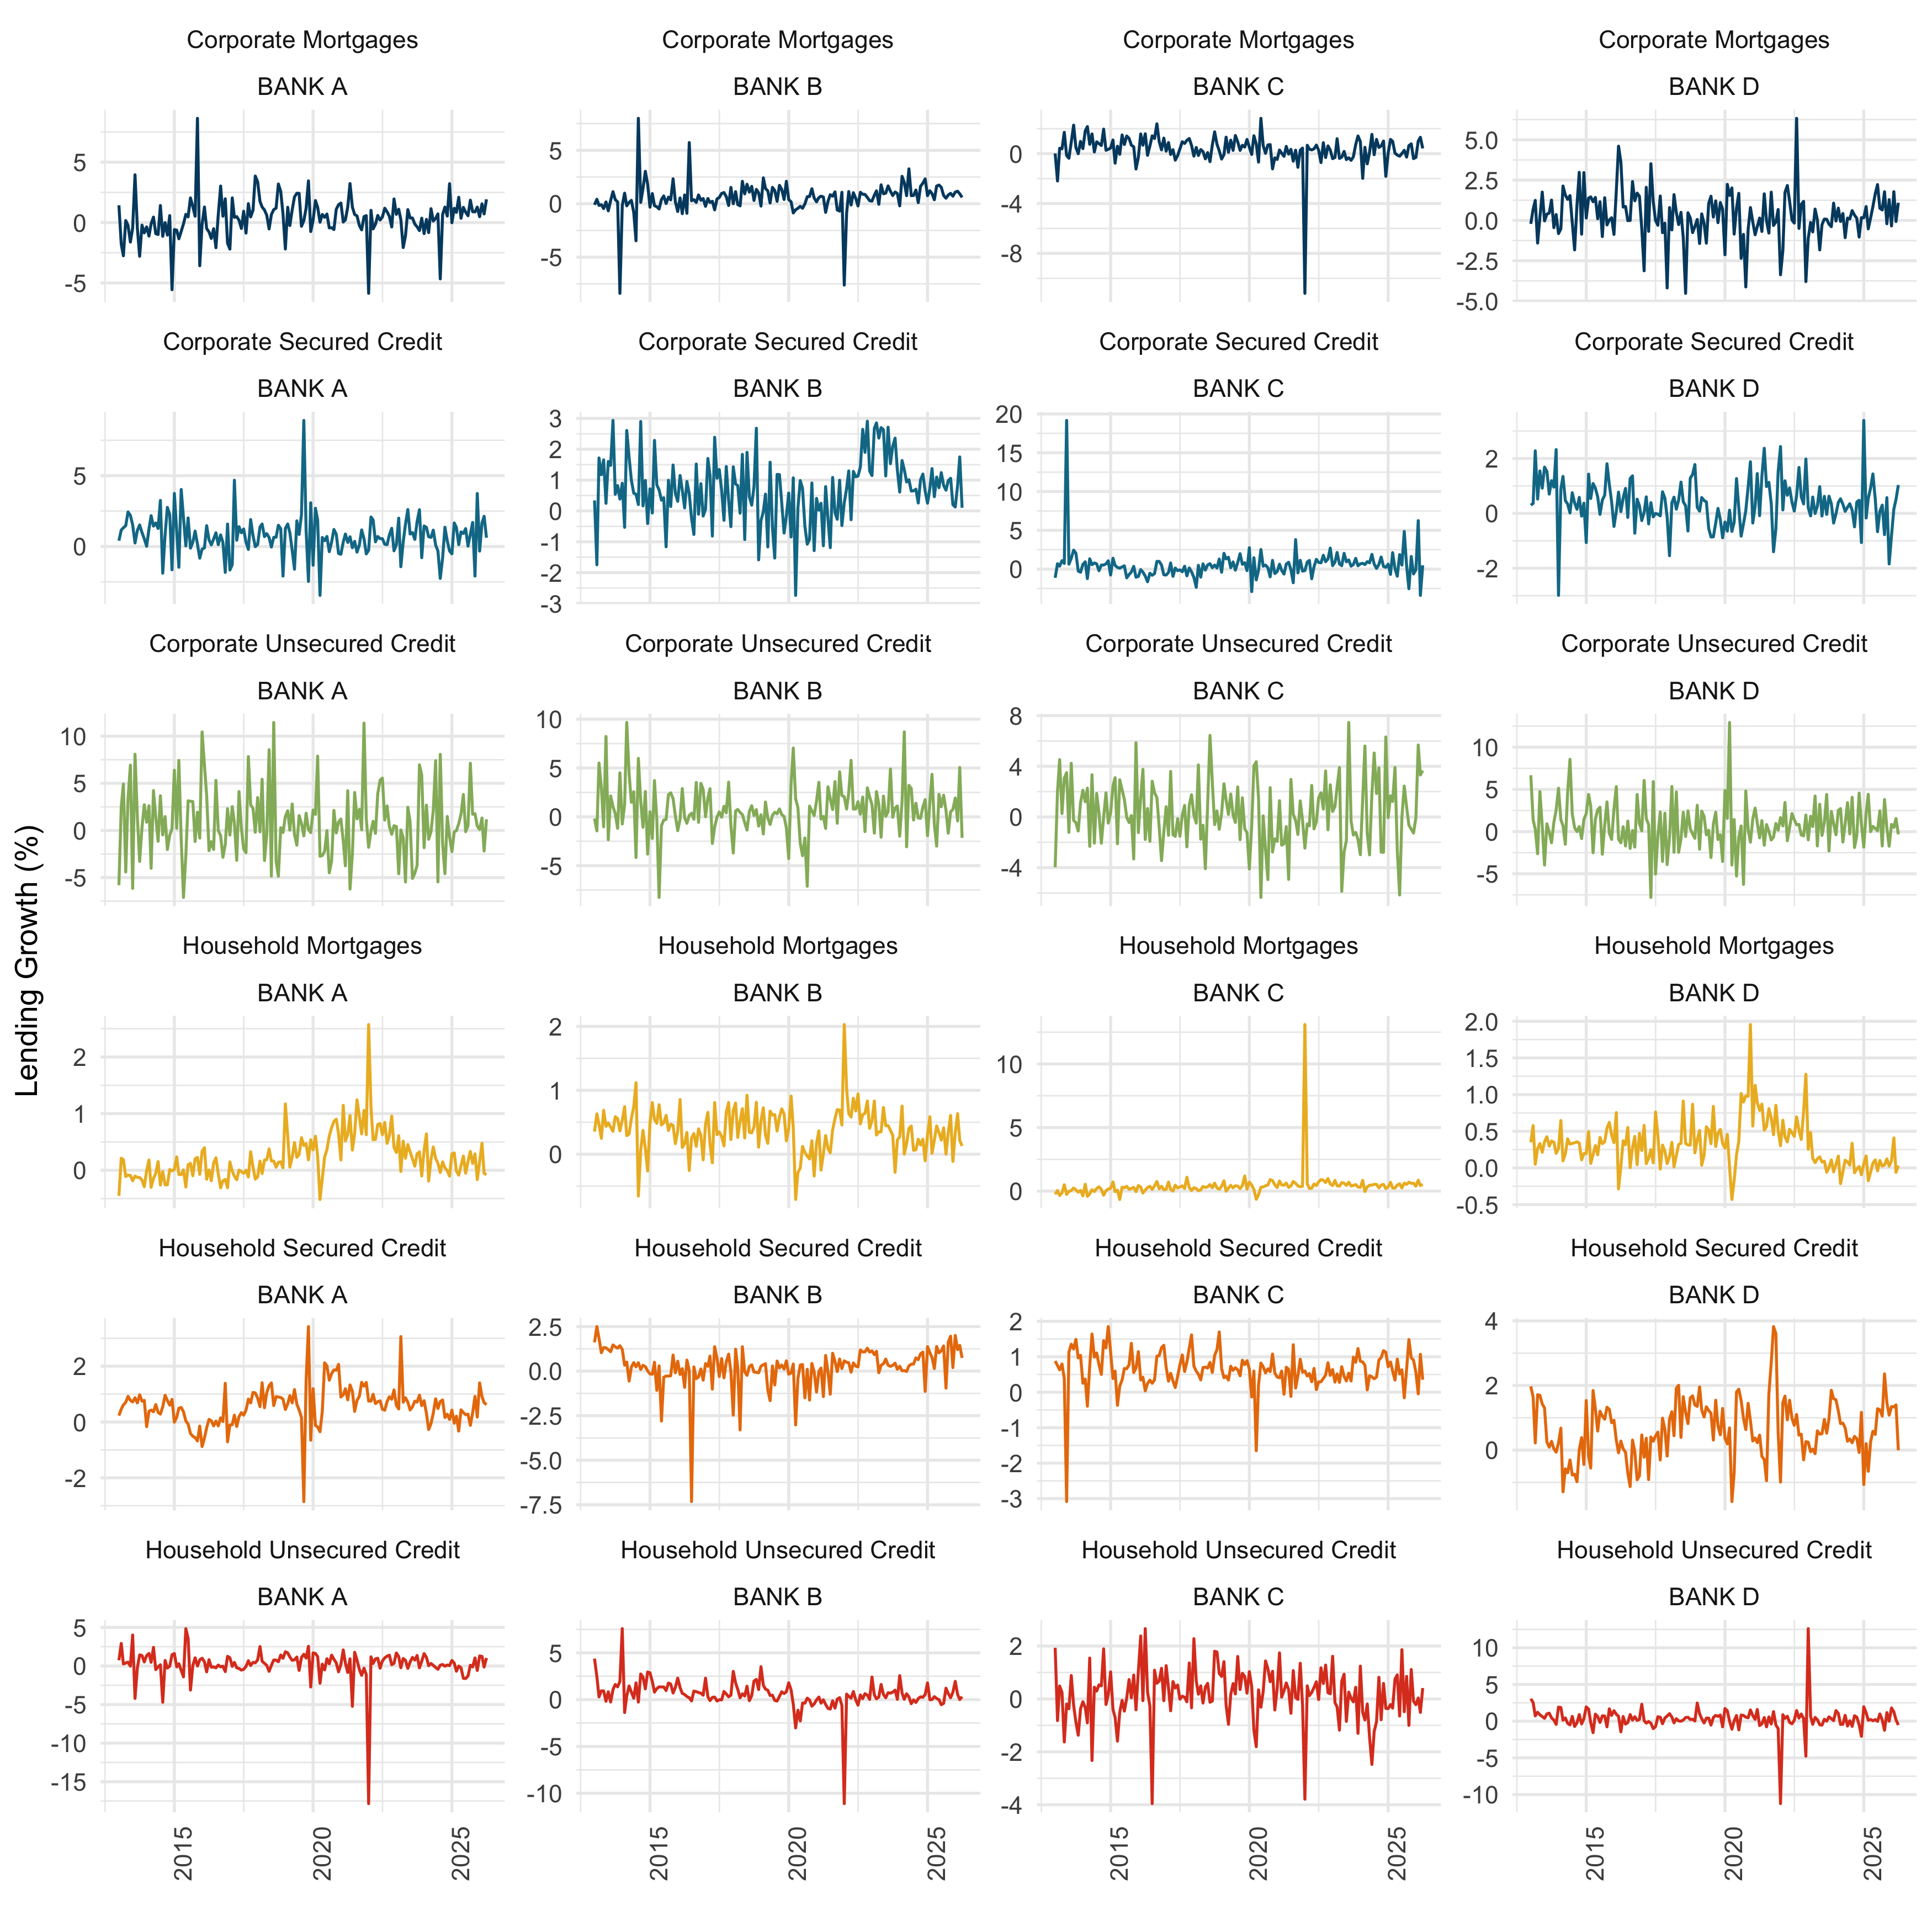
\includegraphics{climate_credit_channel_files/figure-pdf/fig-lending_volume_growth_data-1.png}

}

\caption{\label{fig-lending_volume_growth_data}Private sector credit
extension by borrower type and product, 2011--2025}

\end{figure}%

\fignote{Log of quarterly credit extension at the bank level, disaggregated by borrower type (corporate and household) and product category (unsecured, secured, and mortgage credit). Series are constructed from the South African Reserve Bank's BA900 and BA930 bank compliance reports following \citet{sibande2025} and \citet{sibande2025a}. The sample covers the period 2011Q1–2025Q1 and is restricted to the major South African banking groups.}

\begin{figure}[H]

\centering{

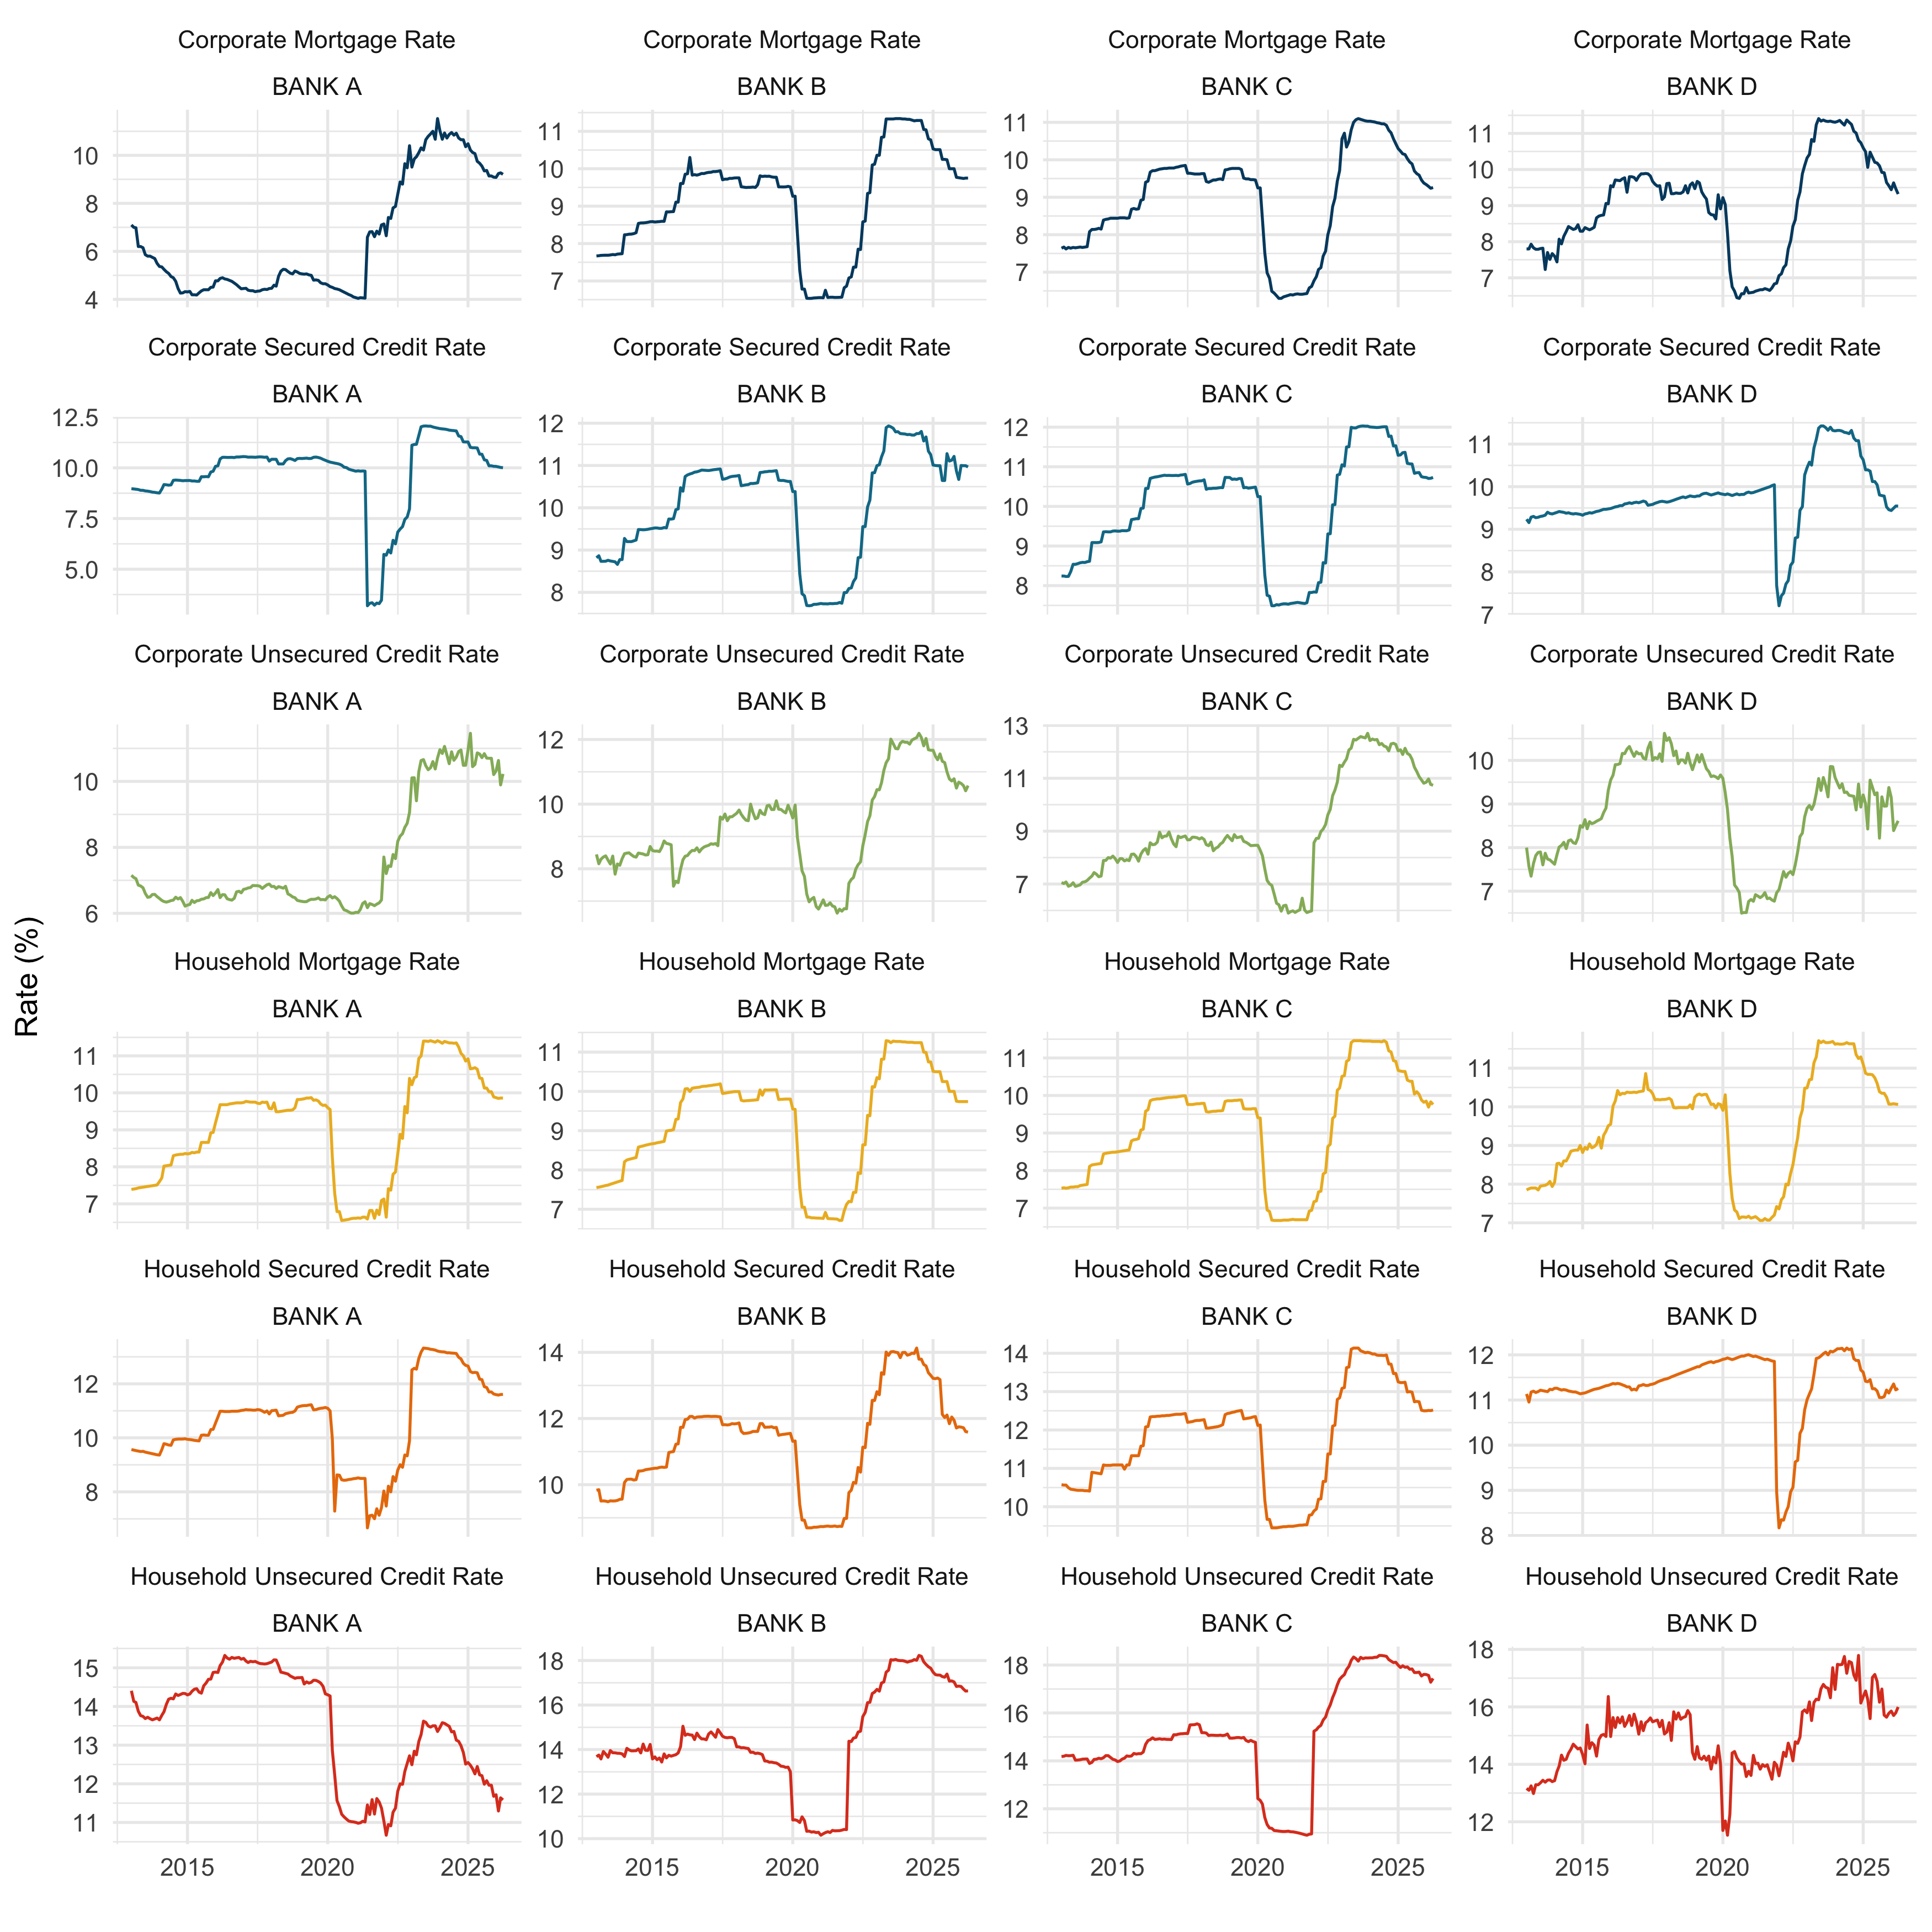
\includegraphics{climate_credit_channel_files/figure-pdf/fig-lending_rates-1.png}

}

\caption{\label{fig-lending_rates}Bank-level lending rates by borrower
type and credit product, 2011--2025}

\end{figure}%

\fignote{Quarterly lending rates at the bank level, disaggregated by borrower type and product (unsecured, secured, and mortgage credit for both corporates and households). Rates are expressed in percentage points and are sourced from the SARB BA930 compliance reports. Unlike credit volumes, lending rates are not log-transformed. The pronounced heterogeneity across banks and products reflects differences in risk pricing, collateral requirements, and borrower characteristics.}

\begin{figure}[H]

\centering{

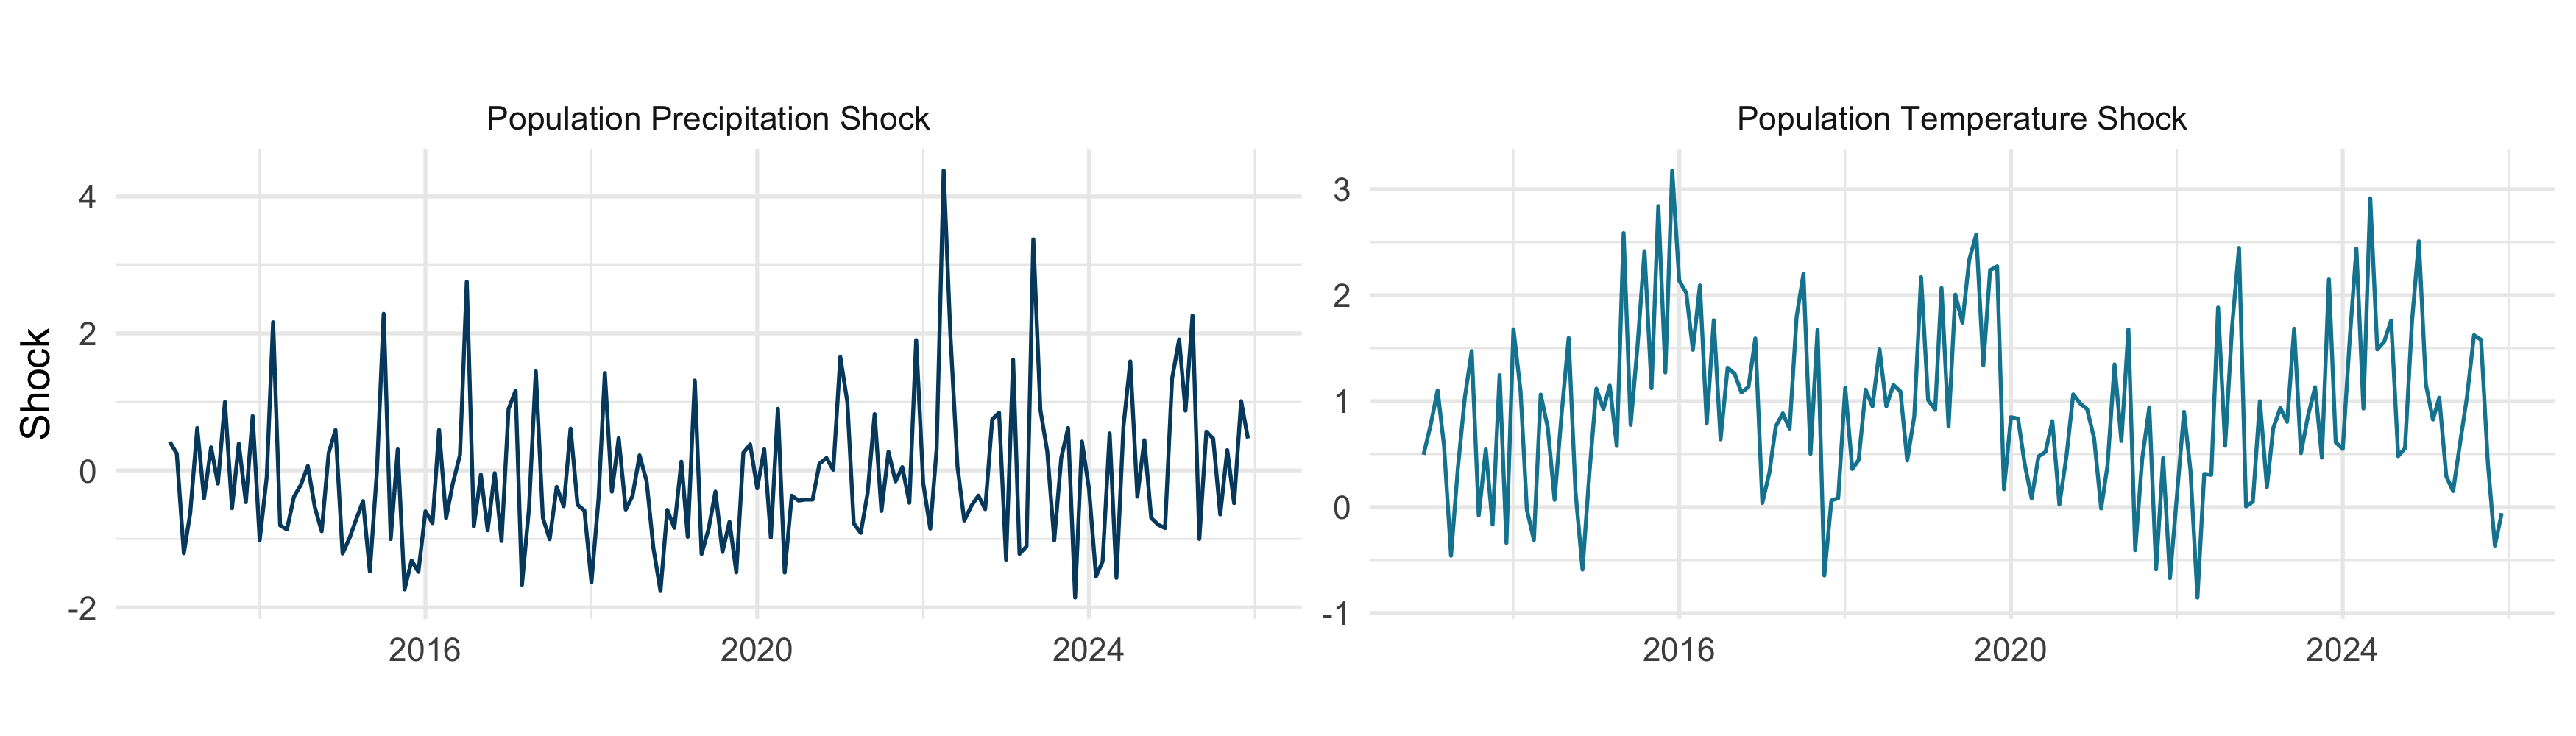
\includegraphics{climate_credit_channel_files/figure-pdf/fig-climate_shocks_data-1.png}

}

\caption{\label{fig-climate_shocks_data}Population-weighted temperature
and precipitation shocks for South Africa, 2011--2025}

\end{figure}%

\fignote{Standardised climate shock series constructed from ERA5 reanalysis data (European Centre for Medium-Range Weather Forecasts) at a 31\,km horizontal resolution. Each observation is the deviation of the population-weighted monthly average from the long-run calendar-month mean, expressed in standard deviation units: $\text{ClimateShock}_t = (T_t - \bar{T}_t)/\sigma(T_t)$. Positive values indicate warmer or wetter conditions than the historical norm; negative values indicate cooler or drier conditions. Grid-level values are weighted by population density and aggregated to a quarterly frequency by averaging within-quarter monthly values.}

\begin{figure}[H]

\centering{

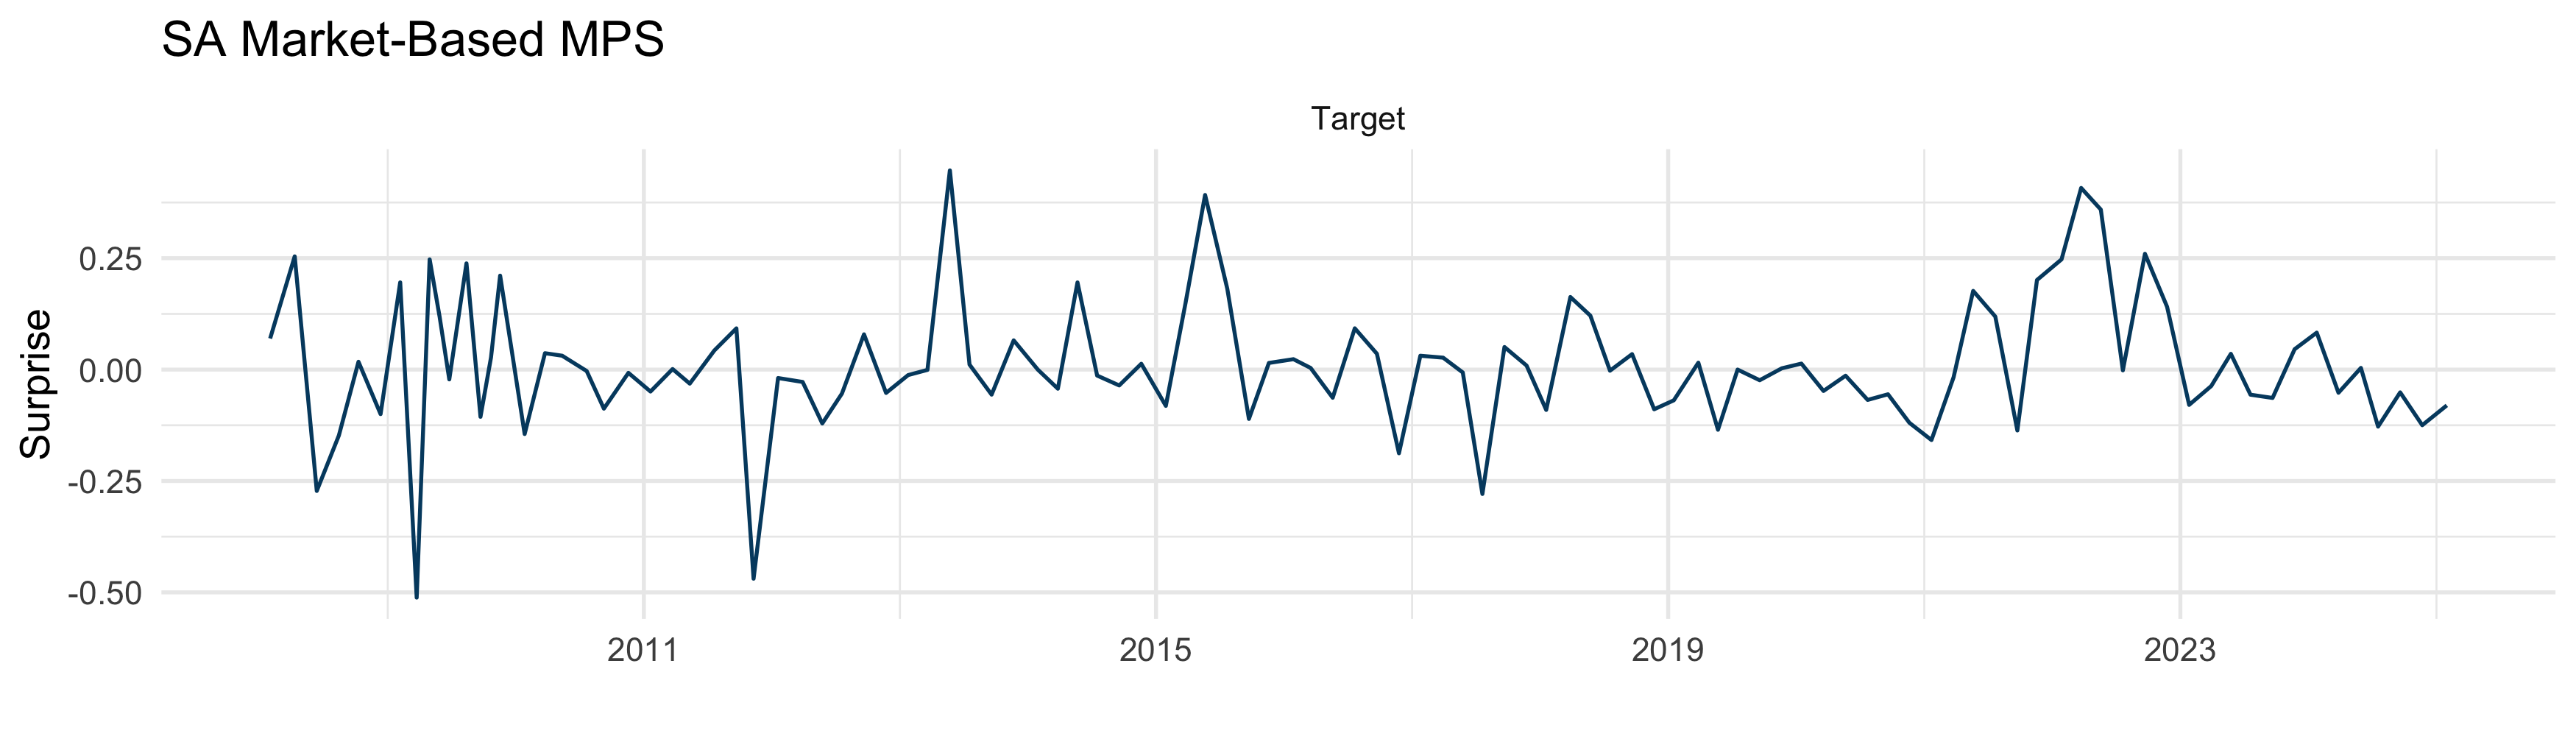
\includegraphics{climate_credit_channel_files/figure-pdf/fig-market_based_surprises_data-1.png}

}

\caption{\label{fig-market_based_surprises_data}High-frequency
market-based monetary policy surprise factors, 2011--2025}

\end{figure}%

\fignote{Monetary policy surprise factors derived from the high-frequency identification approach of \citet{gurkaynak2005} and constructed for South Africa by \citet{pirozhkova2025}. Each factor is extracted from movements in financial market prices in a narrow window around Monetary Policy Committee (MPC) announcement dates. Four components are shown: the \textit{target factor} (surprise in the level of the policy rate), the \textit{forward guidance factor} (surprise in the expected future path of policy), the \textit{central bank information factor} (economic outlook news revealed by the central bank's communication), and the \textit{country risk factor} (shifts in sovereign risk perceptions around MPC dates). Series are aggregated to a quarterly frequency.}

\begin{figure}[H]

\centering{

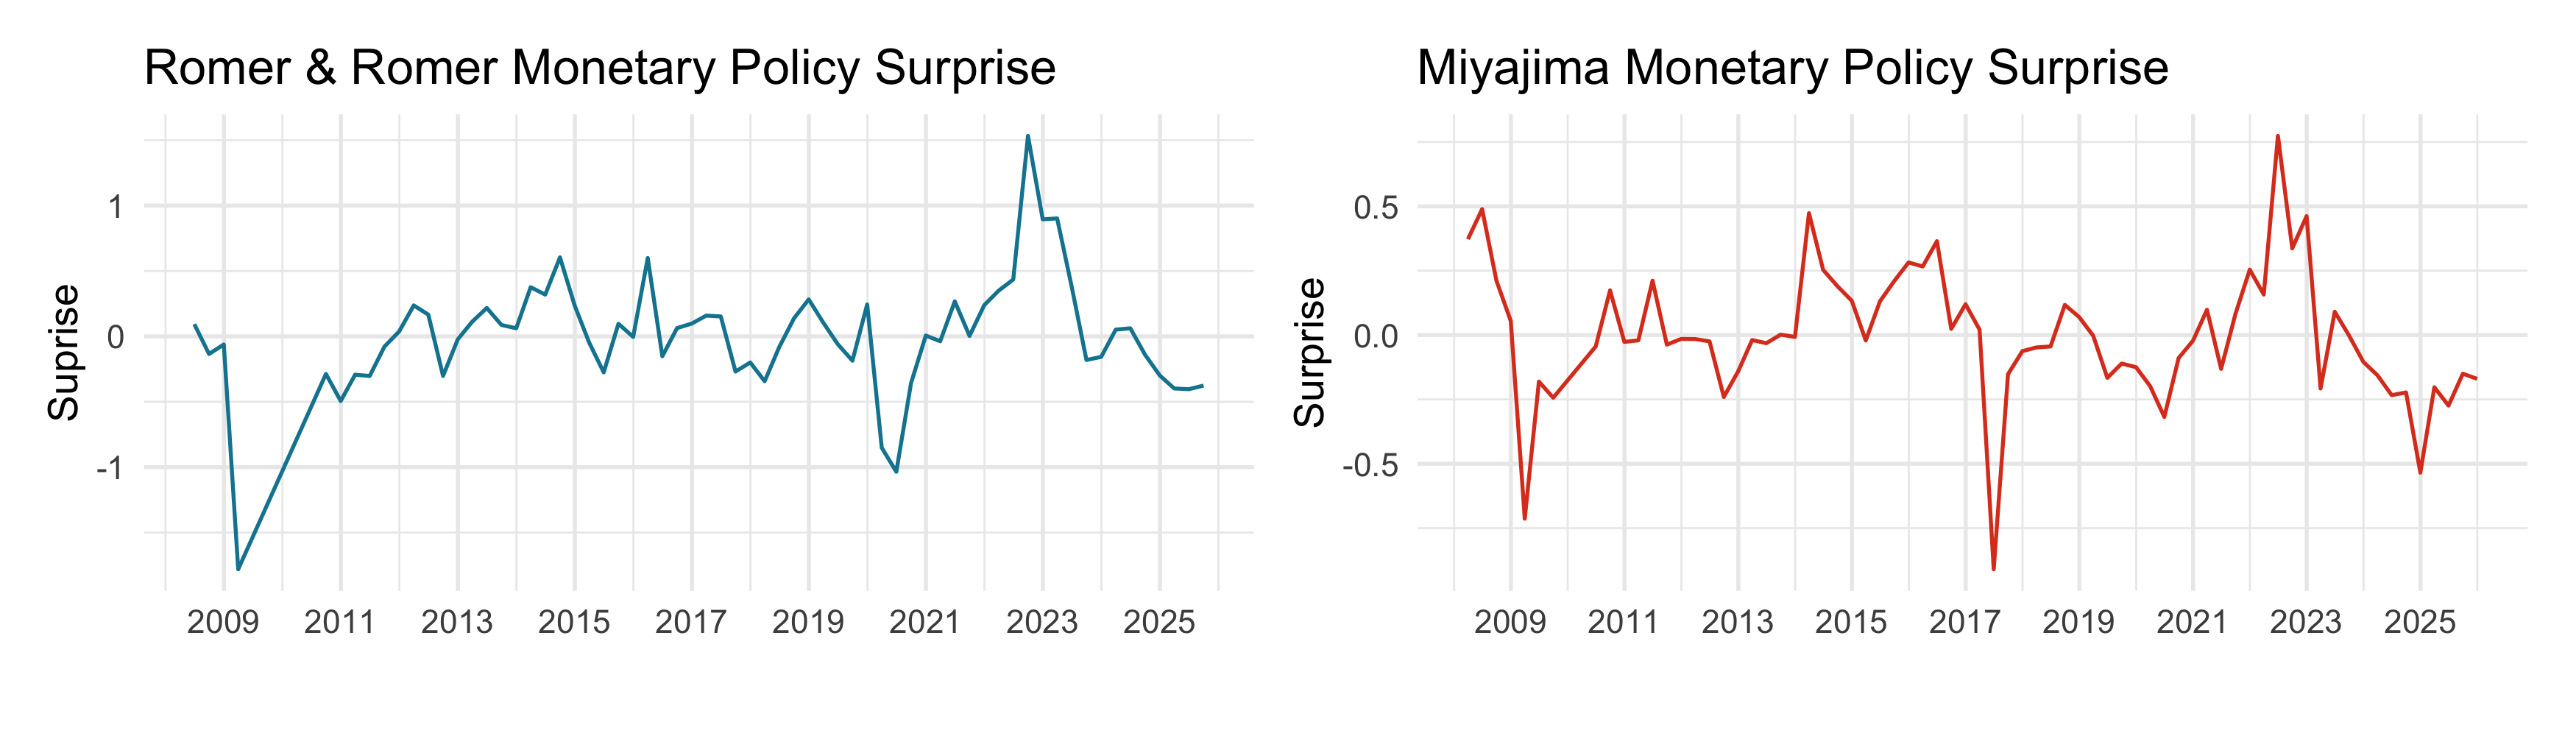
\includegraphics{climate_credit_channel_files/figure-pdf/fig-theory_based_surprises_data-1.png}

}

\caption{\label{fig-theory_based_surprises_data}Theory-based monetary
policy surprises: Romer--Romer and Miyajima measures, 2011--2025}

\end{figure}%

\fignote{Two theory-based monetary policy surprise measures used as alternative identification strategies. The \textit{Romer measure} (blue) is the residual from regressing the change in the SARB's repo rate forecast on its own internal projections for GDP growth and inflation, following the approach of \citet{romer2004} adapted to South Africa by \citet{merrino2022}; a positive value indicates an unexpected tightening relative to the SARB's own information set. The \textit{Miyajima measure} (red) is the residual from regressing the Bloomberg consensus forecast error for the policy rate on forecast errors for inflation and GDP growth \citep{miyajima2024}; a positive value indicates the repo rate came in above what economic news alone would have predicted. Both series are aggregated to a quarterly frequency and purged of climate shock variation prior to use in the main regressions (see Equation~\ref{eq-purge}).}

\subsection{Descriptive Statistics}\label{descriptive-statistics}

\global\setlength{\Oldarrayrulewidth}{\arrayrulewidth}

\global\setlength{\Oldtabcolsep}{\tabcolsep}

\setlength{\tabcolsep}{2pt}

\renewcommand*{\arraystretch}{0.4}



\providecommand{\ascline}[3]{\noalign{\global\arrayrulewidth #1}\arrayrulecolor[HTML]{#2}\cline{#3}}

\begin{longtable}[l]{|p{0.75in}|p{1.50in}|p{0.60in}|p{0.60in}|p{0.60in}|p{0.60in}|p{0.60in}|p{0.50in}}

\caption{\label{tbl-descriptives}Summary statistics for key variables
used in the analysis}

\tabularnewline

\ascline{1pt}{000000}{1-8}

\multicolumn{1}{>{\raggedright}m{\dimexpr 0.75in+0\tabcolsep}}{\advance\leftskip by 5.0pt\relax \advance\rightskip by 5.0pt\relax \textcolor[HTML]{000000}{\fontsize{7}{7}\selectfont{{\fontspec{Arial} }}}} & \multicolumn{1}{>{\raggedright}m{\dimexpr 1.5in+0\tabcolsep}}{\advance\leftskip by 5.0pt\relax \advance\rightskip by 5.0pt\relax \textcolor[HTML]{000000}{\fontsize{7}{7}\selectfont{{\fontspec{Arial} Variable}}}} & \multicolumn{1}{>{\raggedleft}m{\dimexpr 0.6in+0\tabcolsep}}{\advance\leftskip by 5.0pt\relax \advance\rightskip by 5.0pt\relax \textcolor[HTML]{000000}{\fontsize{7}{7}\selectfont{{\fontspec{Arial} Mean}}}} & \multicolumn{1}{>{\raggedleft}m{\dimexpr 0.6in+0\tabcolsep}}{\advance\leftskip by 5.0pt\relax \advance\rightskip by 5.0pt\relax \textcolor[HTML]{000000}{\fontsize{7}{7}\selectfont{{\fontspec{Arial} Median}}}} & \multicolumn{1}{>{\raggedleft}m{\dimexpr 0.6in+0\tabcolsep}}{\advance\leftskip by 5.0pt\relax \advance\rightskip by 5.0pt\relax \textcolor[HTML]{000000}{\fontsize{7}{7}\selectfont{{\fontspec{Arial} SD}}}} & \multicolumn{1}{>{\raggedleft}m{\dimexpr 0.6in+0\tabcolsep}}{\advance\leftskip by 5.0pt\relax \advance\rightskip by 5.0pt\relax \textcolor[HTML]{000000}{\fontsize{7}{7}\selectfont{{\fontspec{Arial} Min}}}} & \multicolumn{1}{>{\raggedleft}m{\dimexpr 0.6in+0\tabcolsep}}{\advance\leftskip by 5.0pt\relax \advance\rightskip by 5.0pt\relax \textcolor[HTML]{000000}{\fontsize{7}{7}\selectfont{{\fontspec{Arial} Max}}}} & \multicolumn{1}{>{\raggedleft}m{\dimexpr 0.5in+0\tabcolsep}}{\advance\leftskip by 5.0pt\relax \advance\rightskip by 5.0pt\relax \textcolor[HTML]{000000}{\fontsize{7}{7}\selectfont{{\fontspec{Arial} N}}}} \\

\ascline{1pt}{000000}{1-8}\endfirsthead 

\ascline{1pt}{000000}{1-8}

\multicolumn{1}{>{\raggedright}m{\dimexpr 0.75in+0\tabcolsep}}{\advance\leftskip by 5.0pt\relax \advance\rightskip by 5.0pt\relax \textcolor[HTML]{000000}{\fontsize{7}{7}\selectfont{{\fontspec{Arial} }}}} & \multicolumn{1}{>{\raggedright}m{\dimexpr 1.5in+0\tabcolsep}}{\advance\leftskip by 5.0pt\relax \advance\rightskip by 5.0pt\relax \textcolor[HTML]{000000}{\fontsize{7}{7}\selectfont{{\fontspec{Arial} Variable}}}} & \multicolumn{1}{>{\raggedleft}m{\dimexpr 0.6in+0\tabcolsep}}{\advance\leftskip by 5.0pt\relax \advance\rightskip by 5.0pt\relax \textcolor[HTML]{000000}{\fontsize{7}{7}\selectfont{{\fontspec{Arial} Mean}}}} & \multicolumn{1}{>{\raggedleft}m{\dimexpr 0.6in+0\tabcolsep}}{\advance\leftskip by 5.0pt\relax \advance\rightskip by 5.0pt\relax \textcolor[HTML]{000000}{\fontsize{7}{7}\selectfont{{\fontspec{Arial} Median}}}} & \multicolumn{1}{>{\raggedleft}m{\dimexpr 0.6in+0\tabcolsep}}{\advance\leftskip by 5.0pt\relax \advance\rightskip by 5.0pt\relax \textcolor[HTML]{000000}{\fontsize{7}{7}\selectfont{{\fontspec{Arial} SD}}}} & \multicolumn{1}{>{\raggedleft}m{\dimexpr 0.6in+0\tabcolsep}}{\advance\leftskip by 5.0pt\relax \advance\rightskip by 5.0pt\relax \textcolor[HTML]{000000}{\fontsize{7}{7}\selectfont{{\fontspec{Arial} Min}}}} & \multicolumn{1}{>{\raggedleft}m{\dimexpr 0.6in+0\tabcolsep}}{\advance\leftskip by 5.0pt\relax \advance\rightskip by 5.0pt\relax \textcolor[HTML]{000000}{\fontsize{7}{7}\selectfont{{\fontspec{Arial} Max}}}} & \multicolumn{1}{>{\raggedleft}m{\dimexpr 0.5in+0\tabcolsep}}{\advance\leftskip by 5.0pt\relax \advance\rightskip by 5.0pt\relax \textcolor[HTML]{000000}{\fontsize{7}{7}\selectfont{{\fontspec{Arial} N}}}} \\

\ascline{1pt}{000000}{1-8}\endhead



\multicolumn{1}{>{\raggedright}m{\dimexpr 0.75in+0\tabcolsep}}{\advance\leftskip by 5.0pt\relax \advance\rightskip by 5.0pt\relax \textcolor[HTML]{000000}{\fontsize{7}{7}\selectfont{{\fontspec{Arial} Climate\ shock}}}} & \multicolumn{1}{>{\raggedright}m{\dimexpr 1.5in+0\tabcolsep}}{\advance\leftskip by 5.0pt\relax \advance\rightskip by 5.0pt\relax \textcolor[HTML]{000000}{\fontsize{7}{7}\selectfont{{\fontspec{Arial} }}}} & \multicolumn{1}{>{\raggedleft}m{\dimexpr 0.6in+0\tabcolsep}}{\advance\leftskip by 5.0pt\relax \advance\rightskip by 5.0pt\relax \textcolor[HTML]{000000}{\fontsize{7}{7}\selectfont{{\fontspec{Arial} }}}} & \multicolumn{1}{>{\raggedleft}m{\dimexpr 0.6in+0\tabcolsep}}{\advance\leftskip by 5.0pt\relax \advance\rightskip by 5.0pt\relax \textcolor[HTML]{000000}{\fontsize{7}{7}\selectfont{{\fontspec{Arial} }}}} & \multicolumn{1}{>{\raggedleft}m{\dimexpr 0.6in+0\tabcolsep}}{\advance\leftskip by 5.0pt\relax \advance\rightskip by 5.0pt\relax \textcolor[HTML]{000000}{\fontsize{7}{7}\selectfont{{\fontspec{Arial} }}}} & \multicolumn{1}{>{\raggedleft}m{\dimexpr 0.6in+0\tabcolsep}}{\advance\leftskip by 5.0pt\relax \advance\rightskip by 5.0pt\relax \textcolor[HTML]{000000}{\fontsize{7}{7}\selectfont{{\fontspec{Arial} }}}} & \multicolumn{1}{>{\raggedleft}m{\dimexpr 0.6in+0\tabcolsep}}{\advance\leftskip by 5.0pt\relax \advance\rightskip by 5.0pt\relax \textcolor[HTML]{000000}{\fontsize{7}{7}\selectfont{{\fontspec{Arial} }}}} & \multicolumn{1}{>{\raggedleft}m{\dimexpr 0.5in+0\tabcolsep}}{\advance\leftskip by 5.0pt\relax \advance\rightskip by 5.0pt\relax \textcolor[HTML]{000000}{\fontsize{7}{7}\selectfont{{\fontspec{Arial} }}}} \\





\multicolumn{1}{>{\raggedright}m{\dimexpr 0.75in+0\tabcolsep}}{\advance\leftskip by 5.0pt\relax \advance\rightskip by 5.0pt\relax \textcolor[HTML]{000000}{\fontsize{7}{7}\selectfont{{\fontspec{Arial} }}}} & \multicolumn{1}{>{\raggedright}m{\dimexpr 1.5in+0\tabcolsep}}{\advance\leftskip by 5.0pt\relax \advance\rightskip by 5.0pt\relax \textcolor[HTML]{000000}{\fontsize{7}{7}\selectfont{{\fontspec{Arial} Population\ Precipitation\ Shock}}}} & \multicolumn{1}{>{\raggedleft}m{\dimexpr 0.6in+0\tabcolsep}}{\advance\leftskip by 5.0pt\relax \advance\rightskip by 5.0pt\relax \textcolor[HTML]{000000}{\fontsize{7}{7}\selectfont{{\fontspec{Arial} -0.26}}}} & \multicolumn{1}{>{\raggedleft}m{\dimexpr 0.6in+0\tabcolsep}}{\advance\leftskip by 5.0pt\relax \advance\rightskip by 5.0pt\relax \textcolor[HTML]{000000}{\fontsize{7}{7}\selectfont{{\fontspec{Arial} -0.48}}}} & \multicolumn{1}{>{\raggedleft}m{\dimexpr 0.6in+0\tabcolsep}}{\advance\leftskip by 5.0pt\relax \advance\rightskip by 5.0pt\relax \textcolor[HTML]{000000}{\fontsize{7}{7}\selectfont{{\fontspec{Arial} 1.88}}}} & \multicolumn{1}{>{\raggedleft}m{\dimexpr 0.6in+0\tabcolsep}}{\advance\leftskip by 5.0pt\relax \advance\rightskip by 5.0pt\relax \textcolor[HTML]{000000}{\fontsize{7}{7}\selectfont{{\fontspec{Arial} -4.54}}}} & \multicolumn{1}{>{\raggedleft}m{\dimexpr 0.6in+0\tabcolsep}}{\advance\leftskip by 5.0pt\relax \advance\rightskip by 5.0pt\relax \textcolor[HTML]{000000}{\fontsize{7}{7}\selectfont{{\fontspec{Arial} 6.38}}}} & \multicolumn{1}{>{\raggedleft}m{\dimexpr 0.5in+0\tabcolsep}}{\advance\leftskip by 5.0pt\relax \advance\rightskip by 5.0pt\relax \textcolor[HTML]{000000}{\fontsize{7}{7}\selectfont{{\fontspec{Arial} 204}}}} \\





\multicolumn{1}{>{\raggedright}m{\dimexpr 0.75in+0\tabcolsep}}{\advance\leftskip by 5.0pt\relax \advance\rightskip by 5.0pt\relax \textcolor[HTML]{000000}{\fontsize{7}{7}\selectfont{{\fontspec{Arial} }}}} & \multicolumn{1}{>{\raggedright}m{\dimexpr 1.5in+0\tabcolsep}}{\advance\leftskip by 5.0pt\relax \advance\rightskip by 5.0pt\relax \textcolor[HTML]{000000}{\fontsize{7}{7}\selectfont{{\fontspec{Arial} Population\ Temperature\ Shock}}}} & \multicolumn{1}{>{\raggedleft}m{\dimexpr 0.6in+0\tabcolsep}}{\advance\leftskip by 5.0pt\relax \advance\rightskip by 5.0pt\relax \textcolor[HTML]{000000}{\fontsize{7}{7}\selectfont{{\fontspec{Arial} 0.96}}}} & \multicolumn{1}{>{\raggedleft}m{\dimexpr 0.6in+0\tabcolsep}}{\advance\leftskip by 5.0pt\relax \advance\rightskip by 5.0pt\relax \textcolor[HTML]{000000}{\fontsize{7}{7}\selectfont{{\fontspec{Arial} 0.88}}}} & \multicolumn{1}{>{\raggedleft}m{\dimexpr 0.6in+0\tabcolsep}}{\advance\leftskip by 5.0pt\relax \advance\rightskip by 5.0pt\relax \textcolor[HTML]{000000}{\fontsize{7}{7}\selectfont{{\fontspec{Arial} 0.69}}}} & \multicolumn{1}{>{\raggedleft}m{\dimexpr 0.6in+0\tabcolsep}}{\advance\leftskip by 5.0pt\relax \advance\rightskip by 5.0pt\relax \textcolor[HTML]{000000}{\fontsize{7}{7}\selectfont{{\fontspec{Arial} -0.59}}}} & \multicolumn{1}{>{\raggedleft}m{\dimexpr 0.6in+0\tabcolsep}}{\advance\leftskip by 5.0pt\relax \advance\rightskip by 5.0pt\relax \textcolor[HTML]{000000}{\fontsize{7}{7}\selectfont{{\fontspec{Arial} 2.84}}}} & \multicolumn{1}{>{\raggedleft}m{\dimexpr 0.5in+0\tabcolsep}}{\advance\leftskip by 5.0pt\relax \advance\rightskip by 5.0pt\relax \textcolor[HTML]{000000}{\fontsize{7}{7}\selectfont{{\fontspec{Arial} 204}}}} \\





\multicolumn{1}{>{\raggedright}m{\dimexpr 0.75in+0\tabcolsep}}{\advance\leftskip by 5.0pt\relax \advance\rightskip by 5.0pt\relax \textcolor[HTML]{000000}{\fontsize{7}{7}\selectfont{{\fontspec{Arial} Lending\ rates}}}} & \multicolumn{1}{>{\raggedright}m{\dimexpr 1.5in+0\tabcolsep}}{\advance\leftskip by 5.0pt\relax \advance\rightskip by 5.0pt\relax \textcolor[HTML]{000000}{\fontsize{7}{7}\selectfont{{\fontspec{Arial} }}}} & \multicolumn{1}{>{\raggedleft}m{\dimexpr 0.6in+0\tabcolsep}}{\advance\leftskip by 5.0pt\relax \advance\rightskip by 5.0pt\relax \textcolor[HTML]{000000}{\fontsize{7}{7}\selectfont{{\fontspec{Arial} }}}} & \multicolumn{1}{>{\raggedleft}m{\dimexpr 0.6in+0\tabcolsep}}{\advance\leftskip by 5.0pt\relax \advance\rightskip by 5.0pt\relax \textcolor[HTML]{000000}{\fontsize{7}{7}\selectfont{{\fontspec{Arial} }}}} & \multicolumn{1}{>{\raggedleft}m{\dimexpr 0.6in+0\tabcolsep}}{\advance\leftskip by 5.0pt\relax \advance\rightskip by 5.0pt\relax \textcolor[HTML]{000000}{\fontsize{7}{7}\selectfont{{\fontspec{Arial} }}}} & \multicolumn{1}{>{\raggedleft}m{\dimexpr 0.6in+0\tabcolsep}}{\advance\leftskip by 5.0pt\relax \advance\rightskip by 5.0pt\relax \textcolor[HTML]{000000}{\fontsize{7}{7}\selectfont{{\fontspec{Arial} }}}} & \multicolumn{1}{>{\raggedleft}m{\dimexpr 0.6in+0\tabcolsep}}{\advance\leftskip by 5.0pt\relax \advance\rightskip by 5.0pt\relax \textcolor[HTML]{000000}{\fontsize{7}{7}\selectfont{{\fontspec{Arial} }}}} & \multicolumn{1}{>{\raggedleft}m{\dimexpr 0.5in+0\tabcolsep}}{\advance\leftskip by 5.0pt\relax \advance\rightskip by 5.0pt\relax \textcolor[HTML]{000000}{\fontsize{7}{7}\selectfont{{\fontspec{Arial} }}}} \\





\multicolumn{1}{>{\raggedright}m{\dimexpr 0.75in+0\tabcolsep}}{\advance\leftskip by 5.0pt\relax \advance\rightskip by 5.0pt\relax \textcolor[HTML]{000000}{\fontsize{7}{7}\selectfont{{\fontspec{Arial} }}}} & \multicolumn{1}{>{\raggedright}m{\dimexpr 1.5in+0\tabcolsep}}{\advance\leftskip by 5.0pt\relax \advance\rightskip by 5.0pt\relax \textcolor[HTML]{000000}{\fontsize{7}{7}\selectfont{{\fontspec{Arial} Corporate\ Mortgage\ Rate}}}} & \multicolumn{1}{>{\raggedleft}m{\dimexpr 0.6in+0\tabcolsep}}{\advance\leftskip by 5.0pt\relax \advance\rightskip by 5.0pt\relax \textcolor[HTML]{000000}{\fontsize{7}{7}\selectfont{{\fontspec{Arial} 8.43}}}} & \multicolumn{1}{>{\raggedleft}m{\dimexpr 0.6in+0\tabcolsep}}{\advance\leftskip by 5.0pt\relax \advance\rightskip by 5.0pt\relax \textcolor[HTML]{000000}{\fontsize{7}{7}\selectfont{{\fontspec{Arial} 9.07}}}} & \multicolumn{1}{>{\raggedleft}m{\dimexpr 0.6in+0\tabcolsep}}{\advance\leftskip by 5.0pt\relax \advance\rightskip by 5.0pt\relax \textcolor[HTML]{000000}{\fontsize{7}{7}\selectfont{{\fontspec{Arial} 2.04}}}} & \multicolumn{1}{>{\raggedleft}m{\dimexpr 0.6in+0\tabcolsep}}{\advance\leftskip by 5.0pt\relax \advance\rightskip by 5.0pt\relax \textcolor[HTML]{000000}{\fontsize{7}{7}\selectfont{{\fontspec{Arial} 4.06}}}} & \multicolumn{1}{>{\raggedleft}m{\dimexpr 0.6in+0\tabcolsep}}{\advance\leftskip by 5.0pt\relax \advance\rightskip by 5.0pt\relax \textcolor[HTML]{000000}{\fontsize{7}{7}\selectfont{{\fontspec{Arial} 11.35}}}} & \multicolumn{1}{>{\raggedleft}m{\dimexpr 0.5in+0\tabcolsep}}{\advance\leftskip by 5.0pt\relax \advance\rightskip by 5.0pt\relax \textcolor[HTML]{000000}{\fontsize{7}{7}\selectfont{{\fontspec{Arial} 212}}}} \\





\multicolumn{1}{>{\raggedright}m{\dimexpr 0.75in+0\tabcolsep}}{\advance\leftskip by 5.0pt\relax \advance\rightskip by 5.0pt\relax \textcolor[HTML]{000000}{\fontsize{7}{7}\selectfont{{\fontspec{Arial} }}}} & \multicolumn{1}{>{\raggedright}m{\dimexpr 1.5in+0\tabcolsep}}{\advance\leftskip by 5.0pt\relax \advance\rightskip by 5.0pt\relax \textcolor[HTML]{000000}{\fontsize{7}{7}\selectfont{{\fontspec{Arial} Corporate\ Secured\ Credit\ Rate}}}} & \multicolumn{1}{>{\raggedleft}m{\dimexpr 0.6in+0\tabcolsep}}{\advance\leftskip by 5.0pt\relax \advance\rightskip by 5.0pt\relax \textcolor[HTML]{000000}{\fontsize{7}{7}\selectfont{{\fontspec{Arial} 9.91}}}} & \multicolumn{1}{>{\raggedleft}m{\dimexpr 0.6in+0\tabcolsep}}{\advance\leftskip by 5.0pt\relax \advance\rightskip by 5.0pt\relax \textcolor[HTML]{000000}{\fontsize{7}{7}\selectfont{{\fontspec{Arial} 9.99}}}} & \multicolumn{1}{>{\raggedleft}m{\dimexpr 0.6in+0\tabcolsep}}{\advance\leftskip by 5.0pt\relax \advance\rightskip by 5.0pt\relax \textcolor[HTML]{000000}{\fontsize{7}{7}\selectfont{{\fontspec{Arial} 1.36}}}} & \multicolumn{1}{>{\raggedleft}m{\dimexpr 0.6in+0\tabcolsep}}{\advance\leftskip by 5.0pt\relax \advance\rightskip by 5.0pt\relax \textcolor[HTML]{000000}{\fontsize{7}{7}\selectfont{{\fontspec{Arial} 3.30}}}} & \multicolumn{1}{>{\raggedleft}m{\dimexpr 0.6in+0\tabcolsep}}{\advance\leftskip by 5.0pt\relax \advance\rightskip by 5.0pt\relax \textcolor[HTML]{000000}{\fontsize{7}{7}\selectfont{{\fontspec{Arial} 12.06}}}} & \multicolumn{1}{>{\raggedleft}m{\dimexpr 0.5in+0\tabcolsep}}{\advance\leftskip by 5.0pt\relax \advance\rightskip by 5.0pt\relax \textcolor[HTML]{000000}{\fontsize{7}{7}\selectfont{{\fontspec{Arial} 212}}}} \\





\multicolumn{1}{>{\raggedright}m{\dimexpr 0.75in+0\tabcolsep}}{\advance\leftskip by 5.0pt\relax \advance\rightskip by 5.0pt\relax \textcolor[HTML]{000000}{\fontsize{7}{7}\selectfont{{\fontspec{Arial} }}}} & \multicolumn{1}{>{\raggedright}m{\dimexpr 1.5in+0\tabcolsep}}{\advance\leftskip by 5.0pt\relax \advance\rightskip by 5.0pt\relax \textcolor[HTML]{000000}{\fontsize{7}{7}\selectfont{{\fontspec{Arial} Corporate\ Unsecured\ Credit\ Rate}}}} & \multicolumn{1}{>{\raggedleft}m{\dimexpr 0.6in+0\tabcolsep}}{\advance\leftskip by 5.0pt\relax \advance\rightskip by 5.0pt\relax \textcolor[HTML]{000000}{\fontsize{7}{7}\selectfont{{\fontspec{Arial} 8.71}}}} & \multicolumn{1}{>{\raggedleft}m{\dimexpr 0.6in+0\tabcolsep}}{\advance\leftskip by 5.0pt\relax \advance\rightskip by 5.0pt\relax \textcolor[HTML]{000000}{\fontsize{7}{7}\selectfont{{\fontspec{Arial} 8.62}}}} & \multicolumn{1}{>{\raggedleft}m{\dimexpr 0.6in+0\tabcolsep}}{\advance\leftskip by 5.0pt\relax \advance\rightskip by 5.0pt\relax \textcolor[HTML]{000000}{\fontsize{7}{7}\selectfont{{\fontspec{Arial} 1.74}}}} & \multicolumn{1}{>{\raggedleft}m{\dimexpr 0.6in+0\tabcolsep}}{\advance\leftskip by 5.0pt\relax \advance\rightskip by 5.0pt\relax \textcolor[HTML]{000000}{\fontsize{7}{7}\selectfont{{\fontspec{Arial} 5.95}}}} & \multicolumn{1}{>{\raggedleft}m{\dimexpr 0.6in+0\tabcolsep}}{\advance\leftskip by 5.0pt\relax \advance\rightskip by 5.0pt\relax \textcolor[HTML]{000000}{\fontsize{7}{7}\selectfont{{\fontspec{Arial} 12.59}}}} & \multicolumn{1}{>{\raggedleft}m{\dimexpr 0.5in+0\tabcolsep}}{\advance\leftskip by 5.0pt\relax \advance\rightskip by 5.0pt\relax \textcolor[HTML]{000000}{\fontsize{7}{7}\selectfont{{\fontspec{Arial} 212}}}} \\





\multicolumn{1}{>{\raggedright}m{\dimexpr 0.75in+0\tabcolsep}}{\advance\leftskip by 5.0pt\relax \advance\rightskip by 5.0pt\relax \textcolor[HTML]{000000}{\fontsize{7}{7}\selectfont{{\fontspec{Arial} }}}} & \multicolumn{1}{>{\raggedright}m{\dimexpr 1.5in+0\tabcolsep}}{\advance\leftskip by 5.0pt\relax \advance\rightskip by 5.0pt\relax \textcolor[HTML]{000000}{\fontsize{7}{7}\selectfont{{\fontspec{Arial} Household\ Mortgage\ Rate}}}} & \multicolumn{1}{>{\raggedleft}m{\dimexpr 0.6in+0\tabcolsep}}{\advance\leftskip by 5.0pt\relax \advance\rightskip by 5.0pt\relax \textcolor[HTML]{000000}{\fontsize{7}{7}\selectfont{{\fontspec{Arial} 9.30}}}} & \multicolumn{1}{>{\raggedleft}m{\dimexpr 0.6in+0\tabcolsep}}{\advance\leftskip by 5.0pt\relax \advance\rightskip by 5.0pt\relax \textcolor[HTML]{000000}{\fontsize{7}{7}\selectfont{{\fontspec{Arial} 9.75}}}} & \multicolumn{1}{>{\raggedleft}m{\dimexpr 0.6in+0\tabcolsep}}{\advance\leftskip by 5.0pt\relax \advance\rightskip by 5.0pt\relax \textcolor[HTML]{000000}{\fontsize{7}{7}\selectfont{{\fontspec{Arial} 1.41}}}} & \multicolumn{1}{>{\raggedleft}m{\dimexpr 0.6in+0\tabcolsep}}{\advance\leftskip by 5.0pt\relax \advance\rightskip by 5.0pt\relax \textcolor[HTML]{000000}{\fontsize{7}{7}\selectfont{{\fontspec{Arial} 6.56}}}} & \multicolumn{1}{>{\raggedleft}m{\dimexpr 0.6in+0\tabcolsep}}{\advance\leftskip by 5.0pt\relax \advance\rightskip by 5.0pt\relax \textcolor[HTML]{000000}{\fontsize{7}{7}\selectfont{{\fontspec{Arial} 11.67}}}} & \multicolumn{1}{>{\raggedleft}m{\dimexpr 0.5in+0\tabcolsep}}{\advance\leftskip by 5.0pt\relax \advance\rightskip by 5.0pt\relax \textcolor[HTML]{000000}{\fontsize{7}{7}\selectfont{{\fontspec{Arial} 212}}}} \\





\multicolumn{1}{>{\raggedright}m{\dimexpr 0.75in+0\tabcolsep}}{\advance\leftskip by 5.0pt\relax \advance\rightskip by 5.0pt\relax \textcolor[HTML]{000000}{\fontsize{7}{7}\selectfont{{\fontspec{Arial} }}}} & \multicolumn{1}{>{\raggedright}m{\dimexpr 1.5in+0\tabcolsep}}{\advance\leftskip by 5.0pt\relax \advance\rightskip by 5.0pt\relax \textcolor[HTML]{000000}{\fontsize{7}{7}\selectfont{{\fontspec{Arial} Household\ Secured\ Credit\ Rate}}}} & \multicolumn{1}{>{\raggedleft}m{\dimexpr 0.6in+0\tabcolsep}}{\advance\leftskip by 5.0pt\relax \advance\rightskip by 5.0pt\relax \textcolor[HTML]{000000}{\fontsize{7}{7}\selectfont{{\fontspec{Arial} 11.28}}}} & \multicolumn{1}{>{\raggedleft}m{\dimexpr 0.6in+0\tabcolsep}}{\advance\leftskip by 5.0pt\relax \advance\rightskip by 5.0pt\relax \textcolor[HTML]{000000}{\fontsize{7}{7}\selectfont{{\fontspec{Arial} 11.35}}}} & \multicolumn{1}{>{\raggedleft}m{\dimexpr 0.6in+0\tabcolsep}}{\advance\leftskip by 5.0pt\relax \advance\rightskip by 5.0pt\relax \textcolor[HTML]{000000}{\fontsize{7}{7}\selectfont{{\fontspec{Arial} 1.42}}}} & \multicolumn{1}{>{\raggedleft}m{\dimexpr 0.6in+0\tabcolsep}}{\advance\leftskip by 5.0pt\relax \advance\rightskip by 5.0pt\relax \textcolor[HTML]{000000}{\fontsize{7}{7}\selectfont{{\fontspec{Arial} 7.09}}}} & \multicolumn{1}{>{\raggedleft}m{\dimexpr 0.6in+0\tabcolsep}}{\advance\leftskip by 5.0pt\relax \advance\rightskip by 5.0pt\relax \textcolor[HTML]{000000}{\fontsize{7}{7}\selectfont{{\fontspec{Arial} 14.11}}}} & \multicolumn{1}{>{\raggedleft}m{\dimexpr 0.5in+0\tabcolsep}}{\advance\leftskip by 5.0pt\relax \advance\rightskip by 5.0pt\relax \textcolor[HTML]{000000}{\fontsize{7}{7}\selectfont{{\fontspec{Arial} 212}}}} \\





\multicolumn{1}{>{\raggedright}m{\dimexpr 0.75in+0\tabcolsep}}{\advance\leftskip by 5.0pt\relax \advance\rightskip by 5.0pt\relax \textcolor[HTML]{000000}{\fontsize{7}{7}\selectfont{{\fontspec{Arial} }}}} & \multicolumn{1}{>{\raggedright}m{\dimexpr 1.5in+0\tabcolsep}}{\advance\leftskip by 5.0pt\relax \advance\rightskip by 5.0pt\relax \textcolor[HTML]{000000}{\fontsize{7}{7}\selectfont{{\fontspec{Arial} Household\ Unsecured\ Credit\ Rate}}}} & \multicolumn{1}{>{\raggedleft}m{\dimexpr 0.6in+0\tabcolsep}}{\advance\leftskip by 5.0pt\relax \advance\rightskip by 5.0pt\relax \textcolor[HTML]{000000}{\fontsize{7}{7}\selectfont{{\fontspec{Arial} 14.52}}}} & \multicolumn{1}{>{\raggedleft}m{\dimexpr 0.6in+0\tabcolsep}}{\advance\leftskip by 5.0pt\relax \advance\rightskip by 5.0pt\relax \textcolor[HTML]{000000}{\fontsize{7}{7}\selectfont{{\fontspec{Arial} 14.54}}}} & \multicolumn{1}{>{\raggedleft}m{\dimexpr 0.6in+0\tabcolsep}}{\advance\leftskip by 5.0pt\relax \advance\rightskip by 5.0pt\relax \textcolor[HTML]{000000}{\fontsize{7}{7}\selectfont{{\fontspec{Arial} 1.96}}}} & \multicolumn{1}{>{\raggedleft}m{\dimexpr 0.6in+0\tabcolsep}}{\advance\leftskip by 5.0pt\relax \advance\rightskip by 5.0pt\relax \textcolor[HTML]{000000}{\fontsize{7}{7}\selectfont{{\fontspec{Arial} 10.22}}}} & \multicolumn{1}{>{\raggedleft}m{\dimexpr 0.6in+0\tabcolsep}}{\advance\leftskip by 5.0pt\relax \advance\rightskip by 5.0pt\relax \textcolor[HTML]{000000}{\fontsize{7}{7}\selectfont{{\fontspec{Arial} 18.37}}}} & \multicolumn{1}{>{\raggedleft}m{\dimexpr 0.5in+0\tabcolsep}}{\advance\leftskip by 5.0pt\relax \advance\rightskip by 5.0pt\relax \textcolor[HTML]{000000}{\fontsize{7}{7}\selectfont{{\fontspec{Arial} 212}}}} \\





\multicolumn{1}{>{\raggedright}m{\dimexpr 0.75in+0\tabcolsep}}{\advance\leftskip by 5.0pt\relax \advance\rightskip by 5.0pt\relax \textcolor[HTML]{000000}{\fontsize{7}{7}\selectfont{{\fontspec{Arial} Log\ of\ credit}}}} & \multicolumn{1}{>{\raggedright}m{\dimexpr 1.5in+0\tabcolsep}}{\advance\leftskip by 5.0pt\relax \advance\rightskip by 5.0pt\relax \textcolor[HTML]{000000}{\fontsize{7}{7}\selectfont{{\fontspec{Arial} }}}} & \multicolumn{1}{>{\raggedleft}m{\dimexpr 0.6in+0\tabcolsep}}{\advance\leftskip by 5.0pt\relax \advance\rightskip by 5.0pt\relax \textcolor[HTML]{000000}{\fontsize{7}{7}\selectfont{{\fontspec{Arial} }}}} & \multicolumn{1}{>{\raggedleft}m{\dimexpr 0.6in+0\tabcolsep}}{\advance\leftskip by 5.0pt\relax \advance\rightskip by 5.0pt\relax \textcolor[HTML]{000000}{\fontsize{7}{7}\selectfont{{\fontspec{Arial} }}}} & \multicolumn{1}{>{\raggedleft}m{\dimexpr 0.6in+0\tabcolsep}}{\advance\leftskip by 5.0pt\relax \advance\rightskip by 5.0pt\relax \textcolor[HTML]{000000}{\fontsize{7}{7}\selectfont{{\fontspec{Arial} }}}} & \multicolumn{1}{>{\raggedleft}m{\dimexpr 0.6in+0\tabcolsep}}{\advance\leftskip by 5.0pt\relax \advance\rightskip by 5.0pt\relax \textcolor[HTML]{000000}{\fontsize{7}{7}\selectfont{{\fontspec{Arial} }}}} & \multicolumn{1}{>{\raggedleft}m{\dimexpr 0.6in+0\tabcolsep}}{\advance\leftskip by 5.0pt\relax \advance\rightskip by 5.0pt\relax \textcolor[HTML]{000000}{\fontsize{7}{7}\selectfont{{\fontspec{Arial} }}}} & \multicolumn{1}{>{\raggedleft}m{\dimexpr 0.5in+0\tabcolsep}}{\advance\leftskip by 5.0pt\relax \advance\rightskip by 5.0pt\relax \textcolor[HTML]{000000}{\fontsize{7}{7}\selectfont{{\fontspec{Arial} }}}} \\





\multicolumn{1}{>{\raggedright}m{\dimexpr 0.75in+0\tabcolsep}}{\advance\leftskip by 5.0pt\relax \advance\rightskip by 5.0pt\relax \textcolor[HTML]{000000}{\fontsize{7}{7}\selectfont{{\fontspec{Arial} }}}} & \multicolumn{1}{>{\raggedright}m{\dimexpr 1.5in+0\tabcolsep}}{\advance\leftskip by 5.0pt\relax \advance\rightskip by 5.0pt\relax \textcolor[HTML]{000000}{\fontsize{7}{7}\selectfont{{\fontspec{Arial} Corporate\ Mortgages}}}} & \multicolumn{1}{>{\raggedleft}m{\dimexpr 0.6in+0\tabcolsep}}{\advance\leftskip by 5.0pt\relax \advance\rightskip by 5.0pt\relax \textcolor[HTML]{000000}{\fontsize{7}{7}\selectfont{{\fontspec{Arial} 25.12}}}} & \multicolumn{1}{>{\raggedleft}m{\dimexpr 0.6in+0\tabcolsep}}{\advance\leftskip by 5.0pt\relax \advance\rightskip by 5.0pt\relax \textcolor[HTML]{000000}{\fontsize{7}{7}\selectfont{{\fontspec{Arial} 25.27}}}} & \multicolumn{1}{>{\raggedleft}m{\dimexpr 0.6in+0\tabcolsep}}{\advance\leftskip by 5.0pt\relax \advance\rightskip by 5.0pt\relax \textcolor[HTML]{000000}{\fontsize{7}{7}\selectfont{{\fontspec{Arial} 0.54}}}} & \multicolumn{1}{>{\raggedleft}m{\dimexpr 0.6in+0\tabcolsep}}{\advance\leftskip by 5.0pt\relax \advance\rightskip by 5.0pt\relax \textcolor[HTML]{000000}{\fontsize{7}{7}\selectfont{{\fontspec{Arial} 23.95}}}} & \multicolumn{1}{>{\raggedleft}m{\dimexpr 0.6in+0\tabcolsep}}{\advance\leftskip by 5.0pt\relax \advance\rightskip by 5.0pt\relax \textcolor[HTML]{000000}{\fontsize{7}{7}\selectfont{{\fontspec{Arial} 25.94}}}} & \multicolumn{1}{>{\raggedleft}m{\dimexpr 0.5in+0\tabcolsep}}{\advance\leftskip by 5.0pt\relax \advance\rightskip by 5.0pt\relax \textcolor[HTML]{000000}{\fontsize{7}{7}\selectfont{{\fontspec{Arial} 212}}}} \\





\multicolumn{1}{>{\raggedright}m{\dimexpr 0.75in+0\tabcolsep}}{\advance\leftskip by 5.0pt\relax \advance\rightskip by 5.0pt\relax \textcolor[HTML]{000000}{\fontsize{7}{7}\selectfont{{\fontspec{Arial} }}}} & \multicolumn{1}{>{\raggedright}m{\dimexpr 1.5in+0\tabcolsep}}{\advance\leftskip by 5.0pt\relax \advance\rightskip by 5.0pt\relax \textcolor[HTML]{000000}{\fontsize{7}{7}\selectfont{{\fontspec{Arial} Corporate\ Secured\ Credit}}}} & \multicolumn{1}{>{\raggedleft}m{\dimexpr 0.6in+0\tabcolsep}}{\advance\leftskip by 5.0pt\relax \advance\rightskip by 5.0pt\relax \textcolor[HTML]{000000}{\fontsize{7}{7}\selectfont{{\fontspec{Arial} 24.17}}}} & \multicolumn{1}{>{\raggedleft}m{\dimexpr 0.6in+0\tabcolsep}}{\advance\leftskip by 5.0pt\relax \advance\rightskip by 5.0pt\relax \textcolor[HTML]{000000}{\fontsize{7}{7}\selectfont{{\fontspec{Arial} 24.22}}}} & \multicolumn{1}{>{\raggedleft}m{\dimexpr 0.6in+0\tabcolsep}}{\advance\leftskip by 5.0pt\relax \advance\rightskip by 5.0pt\relax \textcolor[HTML]{000000}{\fontsize{7}{7}\selectfont{{\fontspec{Arial} 0.37}}}} & \multicolumn{1}{>{\raggedleft}m{\dimexpr 0.6in+0\tabcolsep}}{\advance\leftskip by 5.0pt\relax \advance\rightskip by 5.0pt\relax \textcolor[HTML]{000000}{\fontsize{7}{7}\selectfont{{\fontspec{Arial} 23.38}}}} & \multicolumn{1}{>{\raggedleft}m{\dimexpr 0.6in+0\tabcolsep}}{\advance\leftskip by 5.0pt\relax \advance\rightskip by 5.0pt\relax \textcolor[HTML]{000000}{\fontsize{7}{7}\selectfont{{\fontspec{Arial} 24.95}}}} & \multicolumn{1}{>{\raggedleft}m{\dimexpr 0.5in+0\tabcolsep}}{\advance\leftskip by 5.0pt\relax \advance\rightskip by 5.0pt\relax \textcolor[HTML]{000000}{\fontsize{7}{7}\selectfont{{\fontspec{Arial} 212}}}} \\





\multicolumn{1}{>{\raggedright}m{\dimexpr 0.75in+0\tabcolsep}}{\advance\leftskip by 5.0pt\relax \advance\rightskip by 5.0pt\relax \textcolor[HTML]{000000}{\fontsize{7}{7}\selectfont{{\fontspec{Arial} }}}} & \multicolumn{1}{>{\raggedright}m{\dimexpr 1.5in+0\tabcolsep}}{\advance\leftskip by 5.0pt\relax \advance\rightskip by 5.0pt\relax \textcolor[HTML]{000000}{\fontsize{7}{7}\selectfont{{\fontspec{Arial} Corporate\ Unsecured\ Credit}}}} & \multicolumn{1}{>{\raggedleft}m{\dimexpr 0.6in+0\tabcolsep}}{\advance\leftskip by 5.0pt\relax \advance\rightskip by 5.0pt\relax \textcolor[HTML]{000000}{\fontsize{7}{7}\selectfont{{\fontspec{Arial} 25.75}}}} & \multicolumn{1}{>{\raggedleft}m{\dimexpr 0.6in+0\tabcolsep}}{\advance\leftskip by 5.0pt\relax \advance\rightskip by 5.0pt\relax \textcolor[HTML]{000000}{\fontsize{7}{7}\selectfont{{\fontspec{Arial} 25.73}}}} & \multicolumn{1}{>{\raggedleft}m{\dimexpr 0.6in+0\tabcolsep}}{\advance\leftskip by 5.0pt\relax \advance\rightskip by 5.0pt\relax \textcolor[HTML]{000000}{\fontsize{7}{7}\selectfont{{\fontspec{Arial} 0.28}}}} & \multicolumn{1}{>{\raggedleft}m{\dimexpr 0.6in+0\tabcolsep}}{\advance\leftskip by 5.0pt\relax \advance\rightskip by 5.0pt\relax \textcolor[HTML]{000000}{\fontsize{7}{7}\selectfont{{\fontspec{Arial} 25.04}}}} & \multicolumn{1}{>{\raggedleft}m{\dimexpr 0.6in+0\tabcolsep}}{\advance\leftskip by 5.0pt\relax \advance\rightskip by 5.0pt\relax \textcolor[HTML]{000000}{\fontsize{7}{7}\selectfont{{\fontspec{Arial} 26.42}}}} & \multicolumn{1}{>{\raggedleft}m{\dimexpr 0.5in+0\tabcolsep}}{\advance\leftskip by 5.0pt\relax \advance\rightskip by 5.0pt\relax \textcolor[HTML]{000000}{\fontsize{7}{7}\selectfont{{\fontspec{Arial} 212}}}} \\





\multicolumn{1}{>{\raggedright}m{\dimexpr 0.75in+0\tabcolsep}}{\advance\leftskip by 5.0pt\relax \advance\rightskip by 5.0pt\relax \textcolor[HTML]{000000}{\fontsize{7}{7}\selectfont{{\fontspec{Arial} }}}} & \multicolumn{1}{>{\raggedright}m{\dimexpr 1.5in+0\tabcolsep}}{\advance\leftskip by 5.0pt\relax \advance\rightskip by 5.0pt\relax \textcolor[HTML]{000000}{\fontsize{7}{7}\selectfont{{\fontspec{Arial} Household\ Mortgages}}}} & \multicolumn{1}{>{\raggedleft}m{\dimexpr 0.6in+0\tabcolsep}}{\advance\leftskip by 5.0pt\relax \advance\rightskip by 5.0pt\relax \textcolor[HTML]{000000}{\fontsize{7}{7}\selectfont{{\fontspec{Arial} 26.12}}}} & \multicolumn{1}{>{\raggedleft}m{\dimexpr 0.6in+0\tabcolsep}}{\advance\leftskip by 5.0pt\relax \advance\rightskip by 5.0pt\relax \textcolor[HTML]{000000}{\fontsize{7}{7}\selectfont{{\fontspec{Arial} 26.09}}}} & \multicolumn{1}{>{\raggedleft}m{\dimexpr 0.6in+0\tabcolsep}}{\advance\leftskip by 5.0pt\relax \advance\rightskip by 5.0pt\relax \textcolor[HTML]{000000}{\fontsize{7}{7}\selectfont{{\fontspec{Arial} 0.34}}}} & \multicolumn{1}{>{\raggedleft}m{\dimexpr 0.6in+0\tabcolsep}}{\advance\leftskip by 5.0pt\relax \advance\rightskip by 5.0pt\relax \textcolor[HTML]{000000}{\fontsize{7}{7}\selectfont{{\fontspec{Arial} 25.48}}}} & \multicolumn{1}{>{\raggedleft}m{\dimexpr 0.6in+0\tabcolsep}}{\advance\leftskip by 5.0pt\relax \advance\rightskip by 5.0pt\relax \textcolor[HTML]{000000}{\fontsize{7}{7}\selectfont{{\fontspec{Arial} 26.76}}}} & \multicolumn{1}{>{\raggedleft}m{\dimexpr 0.5in+0\tabcolsep}}{\advance\leftskip by 5.0pt\relax \advance\rightskip by 5.0pt\relax \textcolor[HTML]{000000}{\fontsize{7}{7}\selectfont{{\fontspec{Arial} 212}}}} \\





\multicolumn{1}{>{\raggedright}m{\dimexpr 0.75in+0\tabcolsep}}{\advance\leftskip by 5.0pt\relax \advance\rightskip by 5.0pt\relax \textcolor[HTML]{000000}{\fontsize{7}{7}\selectfont{{\fontspec{Arial} }}}} & \multicolumn{1}{>{\raggedright}m{\dimexpr 1.5in+0\tabcolsep}}{\advance\leftskip by 5.0pt\relax \advance\rightskip by 5.0pt\relax \textcolor[HTML]{000000}{\fontsize{7}{7}\selectfont{{\fontspec{Arial} Household\ Secured\ Credit}}}} & \multicolumn{1}{>{\raggedleft}m{\dimexpr 0.6in+0\tabcolsep}}{\advance\leftskip by 5.0pt\relax \advance\rightskip by 5.0pt\relax \textcolor[HTML]{000000}{\fontsize{7}{7}\selectfont{{\fontspec{Arial} 24.97}}}} & \multicolumn{1}{>{\raggedleft}m{\dimexpr 0.6in+0\tabcolsep}}{\advance\leftskip by 5.0pt\relax \advance\rightskip by 5.0pt\relax \textcolor[HTML]{000000}{\fontsize{7}{7}\selectfont{{\fontspec{Arial} 25.10}}}} & \multicolumn{1}{>{\raggedleft}m{\dimexpr 0.6in+0\tabcolsep}}{\advance\leftskip by 5.0pt\relax \advance\rightskip by 5.0pt\relax \textcolor[HTML]{000000}{\fontsize{7}{7}\selectfont{{\fontspec{Arial} 0.44}}}} & \multicolumn{1}{>{\raggedleft}m{\dimexpr 0.6in+0\tabcolsep}}{\advance\leftskip by 5.0pt\relax \advance\rightskip by 5.0pt\relax \textcolor[HTML]{000000}{\fontsize{7}{7}\selectfont{{\fontspec{Arial} 24.03}}}} & \multicolumn{1}{>{\raggedleft}m{\dimexpr 0.6in+0\tabcolsep}}{\advance\leftskip by 5.0pt\relax \advance\rightskip by 5.0pt\relax \textcolor[HTML]{000000}{\fontsize{7}{7}\selectfont{{\fontspec{Arial} 25.82}}}} & \multicolumn{1}{>{\raggedleft}m{\dimexpr 0.5in+0\tabcolsep}}{\advance\leftskip by 5.0pt\relax \advance\rightskip by 5.0pt\relax \textcolor[HTML]{000000}{\fontsize{7}{7}\selectfont{{\fontspec{Arial} 212}}}} \\





\multicolumn{1}{>{\raggedright}m{\dimexpr 0.75in+0\tabcolsep}}{\advance\leftskip by 5.0pt\relax \advance\rightskip by 5.0pt\relax \textcolor[HTML]{000000}{\fontsize{7}{7}\selectfont{{\fontspec{Arial} }}}} & \multicolumn{1}{>{\raggedright}m{\dimexpr 1.5in+0\tabcolsep}}{\advance\leftskip by 5.0pt\relax \advance\rightskip by 5.0pt\relax \textcolor[HTML]{000000}{\fontsize{7}{7}\selectfont{{\fontspec{Arial} Household\ Unsecured\ Credit}}}} & \multicolumn{1}{>{\raggedleft}m{\dimexpr 0.6in+0\tabcolsep}}{\advance\leftskip by 5.0pt\relax \advance\rightskip by 5.0pt\relax \textcolor[HTML]{000000}{\fontsize{7}{7}\selectfont{{\fontspec{Arial} 24.96}}}} & \multicolumn{1}{>{\raggedleft}m{\dimexpr 0.6in+0\tabcolsep}}{\advance\leftskip by 5.0pt\relax \advance\rightskip by 5.0pt\relax \textcolor[HTML]{000000}{\fontsize{7}{7}\selectfont{{\fontspec{Arial} 25.06}}}} & \multicolumn{1}{>{\raggedleft}m{\dimexpr 0.6in+0\tabcolsep}}{\advance\leftskip by 5.0pt\relax \advance\rightskip by 5.0pt\relax \textcolor[HTML]{000000}{\fontsize{7}{7}\selectfont{{\fontspec{Arial} 0.33}}}} & \multicolumn{1}{>{\raggedleft}m{\dimexpr 0.6in+0\tabcolsep}}{\advance\leftskip by 5.0pt\relax \advance\rightskip by 5.0pt\relax \textcolor[HTML]{000000}{\fontsize{7}{7}\selectfont{{\fontspec{Arial} 24.27}}}} & \multicolumn{1}{>{\raggedleft}m{\dimexpr 0.6in+0\tabcolsep}}{\advance\leftskip by 5.0pt\relax \advance\rightskip by 5.0pt\relax \textcolor[HTML]{000000}{\fontsize{7}{7}\selectfont{{\fontspec{Arial} 25.45}}}} & \multicolumn{1}{>{\raggedleft}m{\dimexpr 0.5in+0\tabcolsep}}{\advance\leftskip by 5.0pt\relax \advance\rightskip by 5.0pt\relax \textcolor[HTML]{000000}{\fontsize{7}{7}\selectfont{{\fontspec{Arial} 212}}}} \\





\multicolumn{1}{>{\raggedright}m{\dimexpr 0.75in+0\tabcolsep}}{\advance\leftskip by 5.0pt\relax \advance\rightskip by 5.0pt\relax \textcolor[HTML]{000000}{\fontsize{7}{7}\selectfont{{\fontspec{Arial} Monetary\ policy\ shock}}}} & \multicolumn{1}{>{\raggedright}m{\dimexpr 1.5in+0\tabcolsep}}{\advance\leftskip by 5.0pt\relax \advance\rightskip by 5.0pt\relax \textcolor[HTML]{000000}{\fontsize{7}{7}\selectfont{{\fontspec{Arial} }}}} & \multicolumn{1}{>{\raggedleft}m{\dimexpr 0.6in+0\tabcolsep}}{\advance\leftskip by 5.0pt\relax \advance\rightskip by 5.0pt\relax \textcolor[HTML]{000000}{\fontsize{7}{7}\selectfont{{\fontspec{Arial} }}}} & \multicolumn{1}{>{\raggedleft}m{\dimexpr 0.6in+0\tabcolsep}}{\advance\leftskip by 5.0pt\relax \advance\rightskip by 5.0pt\relax \textcolor[HTML]{000000}{\fontsize{7}{7}\selectfont{{\fontspec{Arial} }}}} & \multicolumn{1}{>{\raggedleft}m{\dimexpr 0.6in+0\tabcolsep}}{\advance\leftskip by 5.0pt\relax \advance\rightskip by 5.0pt\relax \textcolor[HTML]{000000}{\fontsize{7}{7}\selectfont{{\fontspec{Arial} }}}} & \multicolumn{1}{>{\raggedleft}m{\dimexpr 0.6in+0\tabcolsep}}{\advance\leftskip by 5.0pt\relax \advance\rightskip by 5.0pt\relax \textcolor[HTML]{000000}{\fontsize{7}{7}\selectfont{{\fontspec{Arial} }}}} & \multicolumn{1}{>{\raggedleft}m{\dimexpr 0.6in+0\tabcolsep}}{\advance\leftskip by 5.0pt\relax \advance\rightskip by 5.0pt\relax \textcolor[HTML]{000000}{\fontsize{7}{7}\selectfont{{\fontspec{Arial} }}}} & \multicolumn{1}{>{\raggedleft}m{\dimexpr 0.5in+0\tabcolsep}}{\advance\leftskip by 5.0pt\relax \advance\rightskip by 5.0pt\relax \textcolor[HTML]{000000}{\fontsize{7}{7}\selectfont{{\fontspec{Arial} }}}} \\





\multicolumn{1}{>{\raggedright}m{\dimexpr 0.75in+0\tabcolsep}}{\advance\leftskip by 5.0pt\relax \advance\rightskip by 5.0pt\relax \textcolor[HTML]{000000}{\fontsize{7}{7}\selectfont{{\fontspec{Arial} }}}} & \multicolumn{1}{>{\raggedright}m{\dimexpr 1.5in+0\tabcolsep}}{\advance\leftskip by 5.0pt\relax \advance\rightskip by 5.0pt\relax \textcolor[HTML]{000000}{\fontsize{7}{7}\selectfont{{\fontspec{Arial} Miyajima\ Surprise}}}} & \multicolumn{1}{>{\raggedleft}m{\dimexpr 0.6in+0\tabcolsep}}{\advance\leftskip by 5.0pt\relax \advance\rightskip by 5.0pt\relax \textcolor[HTML]{000000}{\fontsize{7}{7}\selectfont{{\fontspec{Arial} 0.00}}}} & \multicolumn{1}{>{\raggedleft}m{\dimexpr 0.6in+0\tabcolsep}}{\advance\leftskip by 5.0pt\relax \advance\rightskip by 5.0pt\relax \textcolor[HTML]{000000}{\fontsize{7}{7}\selectfont{{\fontspec{Arial} -0.01}}}} & \multicolumn{1}{>{\raggedleft}m{\dimexpr 0.6in+0\tabcolsep}}{\advance\leftskip by 5.0pt\relax \advance\rightskip by 5.0pt\relax \textcolor[HTML]{000000}{\fontsize{7}{7}\selectfont{{\fontspec{Arial} 0.26}}}} & \multicolumn{1}{>{\raggedleft}m{\dimexpr 0.6in+0\tabcolsep}}{\advance\leftskip by 5.0pt\relax \advance\rightskip by 5.0pt\relax \textcolor[HTML]{000000}{\fontsize{7}{7}\selectfont{{\fontspec{Arial} -0.91}}}} & \multicolumn{1}{>{\raggedleft}m{\dimexpr 0.6in+0\tabcolsep}}{\advance\leftskip by 5.0pt\relax \advance\rightskip by 5.0pt\relax \textcolor[HTML]{000000}{\fontsize{7}{7}\selectfont{{\fontspec{Arial} 0.77}}}} & \multicolumn{1}{>{\raggedleft}m{\dimexpr 0.5in+0\tabcolsep}}{\advance\leftskip by 5.0pt\relax \advance\rightskip by 5.0pt\relax \textcolor[HTML]{000000}{\fontsize{7}{7}\selectfont{{\fontspec{Arial} 208}}}} \\





\multicolumn{1}{>{\raggedright}m{\dimexpr 0.75in+0\tabcolsep}}{\advance\leftskip by 5.0pt\relax \advance\rightskip by 5.0pt\relax \textcolor[HTML]{000000}{\fontsize{7}{7}\selectfont{{\fontspec{Arial} }}}} & \multicolumn{1}{>{\raggedright}m{\dimexpr 1.5in+0\tabcolsep}}{\advance\leftskip by 5.0pt\relax \advance\rightskip by 5.0pt\relax \textcolor[HTML]{000000}{\fontsize{7}{7}\selectfont{{\fontspec{Arial} Romer\ Surprise}}}} & \multicolumn{1}{>{\raggedleft}m{\dimexpr 0.6in+0\tabcolsep}}{\advance\leftskip by 5.0pt\relax \advance\rightskip by 5.0pt\relax \textcolor[HTML]{000000}{\fontsize{7}{7}\selectfont{{\fontspec{Arial} 0.06}}}} & \multicolumn{1}{>{\raggedleft}m{\dimexpr 0.6in+0\tabcolsep}}{\advance\leftskip by 5.0pt\relax \advance\rightskip by 5.0pt\relax \textcolor[HTML]{000000}{\fontsize{7}{7}\selectfont{{\fontspec{Arial} 0.06}}}} & \multicolumn{1}{>{\raggedleft}m{\dimexpr 0.6in+0\tabcolsep}}{\advance\leftskip by 5.0pt\relax \advance\rightskip by 5.0pt\relax \textcolor[HTML]{000000}{\fontsize{7}{7}\selectfont{{\fontspec{Arial} 0.41}}}} & \multicolumn{1}{>{\raggedleft}m{\dimexpr 0.6in+0\tabcolsep}}{\advance\leftskip by 5.0pt\relax \advance\rightskip by 5.0pt\relax \textcolor[HTML]{000000}{\fontsize{7}{7}\selectfont{{\fontspec{Arial} -1.04}}}} & \multicolumn{1}{>{\raggedleft}m{\dimexpr 0.6in+0\tabcolsep}}{\advance\leftskip by 5.0pt\relax \advance\rightskip by 5.0pt\relax \textcolor[HTML]{000000}{\fontsize{7}{7}\selectfont{{\fontspec{Arial} 1.53}}}} & \multicolumn{1}{>{\raggedleft}m{\dimexpr 0.5in+0\tabcolsep}}{\advance\leftskip by 5.0pt\relax \advance\rightskip by 5.0pt\relax \textcolor[HTML]{000000}{\fontsize{7}{7}\selectfont{{\fontspec{Arial} 204}}}} \\





\multicolumn{1}{>{\raggedright}m{\dimexpr 0.75in+0\tabcolsep}}{\advance\leftskip by 5.0pt\relax \advance\rightskip by 5.0pt\relax \textcolor[HTML]{000000}{\fontsize{7}{7}\selectfont{{\fontspec{Arial} }}}} & \multicolumn{1}{>{\raggedright}m{\dimexpr 1.5in+0\tabcolsep}}{\advance\leftskip by 5.0pt\relax \advance\rightskip by 5.0pt\relax \textcolor[HTML]{000000}{\fontsize{7}{7}\selectfont{{\fontspec{Arial} Target}}}} & \multicolumn{1}{>{\raggedleft}m{\dimexpr 0.6in+0\tabcolsep}}{\advance\leftskip by 5.0pt\relax \advance\rightskip by 5.0pt\relax \textcolor[HTML]{000000}{\fontsize{7}{7}\selectfont{{\fontspec{Arial} 0.03}}}} & \multicolumn{1}{>{\raggedleft}m{\dimexpr 0.6in+0\tabcolsep}}{\advance\leftskip by 5.0pt\relax \advance\rightskip by 5.0pt\relax \textcolor[HTML]{000000}{\fontsize{7}{7}\selectfont{{\fontspec{Arial} 0.01}}}} & \multicolumn{1}{>{\raggedleft}m{\dimexpr 0.6in+0\tabcolsep}}{\advance\leftskip by 5.0pt\relax \advance\rightskip by 5.0pt\relax \textcolor[HTML]{000000}{\fontsize{7}{7}\selectfont{{\fontspec{Arial} 0.13}}}} & \multicolumn{1}{>{\raggedleft}m{\dimexpr 0.6in+0\tabcolsep}}{\advance\leftskip by 5.0pt\relax \advance\rightskip by 5.0pt\relax \textcolor[HTML]{000000}{\fontsize{7}{7}\selectfont{{\fontspec{Arial} -0.19}}}} & \multicolumn{1}{>{\raggedleft}m{\dimexpr 0.6in+0\tabcolsep}}{\advance\leftskip by 5.0pt\relax \advance\rightskip by 5.0pt\relax \textcolor[HTML]{000000}{\fontsize{7}{7}\selectfont{{\fontspec{Arial} 0.45}}}} & \multicolumn{1}{>{\raggedleft}m{\dimexpr 0.5in+0\tabcolsep}}{\advance\leftskip by 5.0pt\relax \advance\rightskip by 5.0pt\relax \textcolor[HTML]{000000}{\fontsize{7}{7}\selectfont{{\fontspec{Arial} 192}}}} \\

\ascline{1pt}{000000}{1-8}


\end{longtable}

\arrayrulecolor[HTML]{000000}

\global\setlength{\arrayrulewidth}{\Oldarrayrulewidth}

\global\setlength{\tabcolsep}{\Oldtabcolsep}

\renewcommand*{\arraystretch}{1}

\fignote{Summary statistics computed over the full estimation sample (2011Q1--2025Q1) at the bank-quarter level. Credit volumes are expressed in log terms; lending rates are in percentage points; climate shocks are standardised deviations from the long-run calendar-month mean (see Equation~\ref{eq-weather_shock}); and monetary policy surprises are expressed in percentage points. The country risk factor, forward guidance factor, and central bank information factor are excluded from this table to preserve space but are included in the main regressions. $N$ denotes the number of non-missing bank-quarter observations.}

\section{Credit growth results}\label{credit-growth-results}

\subsection{Fixed effects}\label{fixed-effects}

\begin{figure}[H]

\centering{

\includegraphics{climate_credit_channel_files/figure-pdf/fig-rates_fe_temp_models-1.png}

}

\caption{\label{fig-rates_fe_temp_models}Interaction between climate and
monetary policy shocks on credit growth: fixed effects estimates}

\end{figure}%

\fignote{Each point shows the estimated coefficient $\hat{\beta}_3$ on the interaction term $\text{ClimateShock} \times \text{MPShock}$ from Equation~\ref{eq-credit}, with 95\% confidence intervals. Teal points indicate statistical significance at the 5\% level; red points are insignificant. Rows correspond to individual log credit volume series disaggregated by borrower type and product; columns correspond to the four monetary policy surprise measures retained after excluding the country risk and central bank information factors. All models include bank and quarter-of-year fixed effects with standard errors clustered at the bank level. Credit volumes are expressed in logarithms so coefficients represent proportional responses.}

\subsection{Local projections}\label{local-projections}

\begin{figure}[H]

\centering{

\includegraphics{climate_credit_channel_files/figure-pdf/fig-corporate_temp-1.png}

}

\caption{\label{fig-corporate_temp}Impulse responses of corporate credit
growth to monetary policy shocks: temperature shock interaction}

\end{figure}%

\fignote{Impulse response functions (IRFs) from panel local projections estimated at horizons $h = 0, \ldots, 12$ quarters following Equation~\ref{eq-panel_credit}. The blue line shows the cumulative response of log corporate credit growth to the monetary policy shock alone ($\hat{\beta}_2$); the red line shows the response when the same shock coincides with the population-weighted temperature shock ($\hat{\beta}_2 + \hat{\beta}_3$). Shaded bands are 68\% and 90\% Driscoll-Kraay confidence intervals. Rows correspond to corporate unsecured, secured, and mortgage credit; columns correspond to the Miyajima, Romer, and Target monetary policy surprise measures.}

\begin{figure}[H]

\centering{

\includegraphics{climate_credit_channel_files/figure-pdf/fig-corporate_precip-1.png}

}

\caption{\label{fig-corporate_precip}Impulse responses of corporate
credit growth to monetary policy shocks: precipitation shock
interaction}

\end{figure}%

\fignote{As Figure~\ref{fig-corporate_temp} but for the population-weighted precipitation shock. The red line shows the corporate credit growth response when the monetary policy shock coincides with a precipitation shock ($\hat{\beta}_2 + \hat{\beta}_3$). Rows correspond to corporate unsecured, secured, and mortgage credit.}

\newpage

\begin{figure}[H]

\centering{

\includegraphics{climate_credit_channel_files/figure-pdf/fig-household_temp-1.png}

}

\caption{\label{fig-household_temp}Impulse responses of household credit
growth to monetary policy shocks: temperature shock interaction}

\end{figure}%

\fignote{As Figure~\ref{fig-corporate_temp} but for household credit growth (unsecured, secured, and mortgage). The gap between the blue and red lines at each horizon represents the marginal effect of the temperature shock on the transmission of monetary policy to household credit volumes.}

\begin{figure}[H]

\centering{

\includegraphics{climate_credit_channel_files/figure-pdf/fig-household_precip-1.png}

}

\caption{\label{fig-household_precip}Impulse responses of household
credit growth to monetary policy shocks: precipitation shock
interaction}

\end{figure}%

\fignote{As Figure~\ref{fig-household_temp} but for the population-weighted precipitation shock. Rows correspond to household unsecured, secured, and mortgage credit growth.}

\subsection{Asymmetric local
projections}\label{asymmetric-local-projections}

\begin{figure}[H]

\centering{

\includegraphics{climate_credit_channel_files/figure-pdf/fig-asym_corporate_temp-1.png}

}

\caption{\label{fig-asym_corporate_temp}Asymmetric impulse responses of
corporate credit growth under extreme temperature states}

\end{figure}%

\fignote{Impulse response functions from asymmetric panel local projections. The blue line shows the cumulative response of log corporate credit growth to the monetary policy shock in the absence of a climate shock; the red line shows the response evaluated at an extreme positive temperature state ($+3$ SD). The gap between the two paths is the marginal climate amplification or dampening effect at that climate intensity. Shaded bands are 68\% and 90\% Driscoll-Kraay confidence intervals. Rows correspond to corporate unsecured, secured, and mortgage credit growth.}

\begin{figure}[H]

\centering{

\includegraphics{climate_credit_channel_files/figure-pdf/fig-asym_corporate_precip-1.png}

}

\caption{\label{fig-asym_corporate_precip}Asymmetric impulse responses
of corporate credit growth under extreme precipitation states}

\end{figure}%

\fignote{As Figure~\ref{fig-asym_corporate_temp} but evaluated at an extreme negative precipitation state ($-3$ SD, i.e.\ drought conditions). A divergence between the red and blue lines indicates that drought conditions amplify or dampen the transmission of monetary policy to corporate credit volumes relative to the no-climate-shock baseline. Rows correspond to corporate unsecured, secured, and mortgage credit growth.}

\newpage

\begin{figure}[H]

\centering{

\includegraphics{climate_credit_channel_files/figure-pdf/fig-asym_household_temp-1.png}

}

\caption{\label{fig-asym_household_temp}Asymmetric impulse responses of
household credit growth under extreme temperature states}

\end{figure}%

\fignote{As Figure~\ref{fig-asym_corporate_temp} but for household credit growth (unsecured, secured, and mortgage). Compares the monetary policy transmission response in the absence of a climate shock against the response under an extreme positive temperature state ($+3$ SD).}

\begin{figure}[H]

\centering{

\includegraphics{climate_credit_channel_files/figure-pdf/fig-asym_household_precip-1.png}

}

\caption{\label{fig-asym_household_precip}Asymmetric impulse responses
of household credit growth under extreme precipitation states}

\end{figure}%

\fignote{As Figure~\ref{fig-asym_household_temp} but evaluated at an extreme negative precipitation state ($-3$ SD). Rows correspond to household unsecured, secured, and mortgage credit growth.}

\newpage


\renewcommand\refname{Credit rates results with controls (to complete)}


\end{document}
